%=================================================================
% Post-Conflict LULC Transitions in Urabá Antioqueño
% Format: article class, APA 7th edition (biblatex + biber)
%=================================================================
\documentclass[12pt,a4paper]{article}

% Language setting
\usepackage[american]{babel}

% Set page size and margins
\usepackage[a4paper,top=2cm,bottom=2cm,left=2.5cm,right=2.5cm,marginparwidth=1.75cm]{geometry}

%----------- APA style references & citations ---
\usepackage[style=apa, backend=biber, natbib=true]{biblatex}
\addbibresource{references.bib}
\DeclareLanguageMapping{american}{american-apa}
\DeclareFieldFormat[article]{volume}{\apanum{#1}}
\renewcommand*{\finalnamedelim}{%
  \ifnumgreater{\value{liststop}}{2}{\finalandcomma}{}%
  \addspace\&\space}

% Math
\usepackage{amsmath}
\usepackage{amsfonts}

% Graphics
\usepackage{graphicx}
\usepackage{subcaption}
\graphicspath{{./figures/}}

% Tables
\usepackage{booktabs}
\usepackage{multirow}
\usepackage{threeparttable}

% Units
\usepackage{siunitx}
\sisetup{group-separator={,}, group-minimum-digits=4, separate-uncertainty=true}

% Fonts and encoding
\usepackage[utf8]{inputenc}
\usepackage[T1]{fontenc}
\DeclareUnicodeCharacter{0301}{\'{}}  % combining acute accent
\usepackage{csquotes}
\usepackage{lmodern}
\usepackage{helvet}

% Hyperlinks
\usepackage[colorlinks=true, allcolors=blue]{hyperref}
\usepackage{url}

% Lists
\usepackage{enumitem}

% Captions and floats
\usepackage{float}
\usepackage[justification=raggedright, singlelinecheck=false]{caption}
\captionsetup[table]{position=top}

% Line spacing
\usepackage{setspace}
\onehalfspacing

% Section formatting
\usepackage{titlesec}
\titleformat{\section}
  {\normalfont\Large\bfseries}{\thesection.}{1em}{}

% Suppress PDF warnings
\pdfsuppresswarningpagegroup=1

\date{}


\begin{document}

%----------
% Title and Authors
%----------

\begin{center}
{\LARGE Post-Conflict Land Use Transitions in Urab\'{a} Antioque\~{n}o, Colombia: A Multi-Temporal Remote Sensing Analysis of Deforestation Drivers and Ecosystem Service Impacts (2013--2024)} \\[5ex]

{\large Cristian Espinal Maya} \\
{\small
School of Finance, Economics and Government, Universidad EAFIT, Medell\'{i}n 050022, Colombia \\
cjespinalm@eafit.edu.co
} \\[1.2em]

{\large Santiago Jim\'{e}nez Londo\~{n}o} \\
{\small
School of Applied Sciences and Engineering, Universidad EAFIT, Medell\'{i}n 050022, Colombia \\
sjimene8@eafit.edu.co
}
\end{center}

\begin{abstract}
Colombia's Urab\'{a} Antioque\~{n}o region---situated at the intersection of the Choc\'{o} biogeographic province, the Caribbean coast, and the Dari\'{e}n Gap---represents one of the most ecologically valuable and conflict-affected territories in the Neotropics. This study analyzes the spatiotemporal dynamics of land use and land cover change (LULCC) across 15 municipalities (${\sim}$11,000~km$^2$) in Urab\'{a} spanning four periods from active conflict through post-agreement implementation (2013--2024). Using Random Forest classification in Google Earth Engine with Landsat~8/9 and Sentinel-2 imagery (12 spectral-topographic features), we produced four LULC maps with eight classes including mangroves---a critical coastal ecosystem providing blue carbon storage. \citet{Olofsson2014} stratified area estimators with 95\% confidence intervals quantified classification uncertainty. Transition matrices and Getis-Ord Gi* hotspot analysis characterized spatial patterns of deforestation, with hotspots concentrated along the Dari\'{e}n frontier and southern montane zone. Total carbon stocks (IPCC Tier~2, calibrated for Choc\'{o} humid tropical forests) were estimated across four pools including mangrove blue carbon (soil C~$= 120$~Mg~C~ha$^{-1}$). Geographically Weighted Regression identified spatially varying drivers of deforestation, with elevation, distance to coast, and proximity to banana/palm plantations as key explanatory variables. CA-Markov projections under three governance scenarios (BAU, Conservation, PDET Urab\'{a}) project divergent forest trajectories to 2040. These findings provide critical inputs for PDET Urab\'{a} territorial planning, mangrove conservation along the Gulf of Urab\'{a}, and land restitution programs in a region marked by paramilitary legacy and ongoing governance challenges, contributing to SDGs~6, 13, 14, 15, and~16.
\end{abstract}

\textbf{Keywords}: Land use/land cover change, Post-conflict deforestation, Ecosystem services, Google Earth Engine, Urab\'{a} Antioque\~{n}o, Choc\'{o} bioregion, Mangroves, Blue carbon, Random Forest, Geographically weighted regression, CA-Markov.


%%%%%%%%%%%%%%%%%%%%%%%%%%%%%%%%%%%%%%%%%%
\section{Introduction}
%%%%%%%%%%%%%%%%%%%%%%%%%%%%%%%%%%%%%%%%%%

\subsection{Armed Conflict and Tropical Deforestation}

Armed conflict exerts profound but paradoxical effects on tropical forests. While active warfare often restricts access to remote areas---creating inadvertent ``gunpoint conservation'' \citep{Alvarez2003}---the cessation of hostilities can trigger rapid deforestation as governance vacuums emerge and previously inaccessible territories become open to agricultural expansion, land speculation, and resource extraction \citep{Prem2020,Clerici2020}. This phenomenon has been documented across multiple post-conflict contexts, from Sierra Leone to Nepal, but nowhere has it been as acutely manifest as in Colombia \citep{Fagan2020,CastroNunez2022,MurilloSandoval2021}.

Colombia's 2016 peace agreement with the FARC-EP guerrilla ended over five decades of internal armed conflict. The environmental consequences were swift and paradoxical: deforestation rates increased by 44\% nationally between 2015 and 2017, with the most pronounced increases occurring in former conflict-affected territories \citep{IDEAM2018,Prem2020}. \citet{Clerici2020} documented a 177\% increase in deforestation rates within and around protected areas in post-conflict zones, while \citet{CastroNunez2022} identified extensive cattle ranching and land speculation---rather than smallholder agriculture---as the primary drivers of forest conversion \citep[see also][]{Pacheco2009,Negret2019}. \citet{Sierra2017} emphasized the urgent need for ecological monitoring systems during Colombia's rapid post-conflict transition.

\subsection{The Post-Conflict Environmental Challenge in Colombia}

Post-conflict environmental dynamics in Colombia have been predominantly studied in the Amazon and Pacific regions \citep{Prem2020,Clerici2020,MurilloSandoval2021,Negret2019}, relying predominantly on the Hansen Global Forest Change dataset \citep{Hansen2013}, which captures only binary forest loss/gain rather than complete land use transitions. This represents a critical knowledge gap: understanding \textit{what replaces forest}---and the spatial patterns of these transitions---is essential for designing effective territorial development strategies and conservation interventions.

The northwestern Colombian region of Urab\'{a} Antioque\~{n}o presents a distinctive and understudied case that differs fundamentally from the Amazonian frontier dynamics that dominate the literature. Unlike the Amazon's colonization-driven deforestation, Urab\'{a}'s land use dynamics are shaped by an established agroindustrial economy (banana, plantain, oil palm), a legacy of paramilitary territorial control, coastal ecosystem degradation, and its role as a critical migration corridor through the Dari\'{e}n Gap.

\subsection{Urab\'{a} Antioque\~{n}o: A Critical and Understudied Landscape}

The Urab\'{a} Antioque\~{n}o region, situated in northwestern Colombia where the Andean cordillera meets the Caribbean coast and the Choc\'{o} biogeographic province, represents one of the most ecologically valuable yet socioeconomically complex landscapes in the Neotropics. The region encompasses approximately 11,000~km$^2$ across 15 municipalities in the departments of Antioquia and Choc\'{o}, bordering the Gulf of Urab\'{a} and the Dari\'{e}n Gap---the only break in the Pan-American Highway connecting Central and South America.

\textbf{Ecological significance.} Urab\'{a} lies within the Choc\'{o}-Dari\'{e}n biodiversity hotspot \citep{Myers2000,Gentry1986}, one of Earth's most biodiverse regions. The Choc\'{o} biogeographic province holds the highest recorded plant diversity per unit area globally \citep{Gentry1986}, and the region supports multiple critical ecosystem types: tropical humid forest with exceptionally high biomass ($>$155~Mg~C~ha$^{-1}$ aboveground; \citealp{Phillips2019,Alvarez2012}), coastal mangrove forests along the Gulf of Urab\'{a} and R\'{i}o Atrato estuary \citep{BlancoLibreros2012,BlancoLibreros2015}, and wetland complexes associated with the Atrato River basin. Mangrove ecosystems are particularly significant for ``blue carbon'' storage, with soil carbon densities reaching 120~Mg~C~ha$^{-1}$ due to anaerobic conditions preventing decomposition \citep{Donato2011,Twilley2018,Alongi2014}.

\textbf{Socioeconomic context.} The region's economy is driven by banana and plantain cultivation for export (managed by associations including Augura and Uniban), oil palm expansion, extensive cattle ranching, artisanal and illegal gold mining, and coca cultivation \citep{Castiblanco2013}. The ``eje bananero'' municipalities (Apartad\'{o}, Carepa, Chigorod\'{o}, Turbo) constitute one of Colombia's most productive agricultural corridors, while peripheral municipalities face subsistence economies and limited state presence.

\textbf{Conflict legacy.} Urab\'{a}'s conflict history is distinct from the FARC-dominated Amazon narrative. The region was the epicenter of paramilitary consolidation in the 1990s, with the Autodefensas Unidas de Colombia (AUC) establishing territorial control through systematic violence, forced displacement, and land appropriation \citep{GarciaDeLaTorre2011,Uribe2001,GutierrezSanin2014}. Following AUC demobilization (2003--2006) under the Ley de Justicia y Paz, successor armed groups---notably the Clan del Golfo (Autodefensas Gaitanistas de Colombia)---filled governance vacuums \citep{Grajales2011,Grajales2015}. Land restitution under Ley 1448 de 2011 has been particularly contentious in Urab\'{a}, where paramilitary-era land dispossession remains partially unresolved \citep{SanchezGomez2020,Thomson2011}. Since 2019, the region has additionally become the primary transit corridor for irregular migration flows from South America through the Dari\'{e}n Gap toward North America.

\textbf{Conservation assets.} The region includes Parque Nacional Natural Los Kat\'{i}os (a UNESCO World Heritage Site protecting Choc\'{o}-Dari\'{e}n forests) and extensive mangrove ecosystems along the Gulf coast that have experienced documented degradation \citep{BlancoLibreros2015,Estrada2014,Polidoro2010}.

\subsection{Remote Sensing for Multi-Temporal LULC Analysis}

Google Earth Engine (GEE) has revolutionized large-area land use classification by providing cloud-based access to multi-petabyte satellite archives with planetary-scale computing power \citep{Gorelick2017}. The availability of five decades of Landsat imagery \citep{Wulder2022} combined with the higher spatial resolution of Sentinel-2 \citep{Drusch2012} enables multi-sensor approaches for improved temporal and spatial coverage. Random Forest (RF) classifiers \citep{Breiman2001} operating within GEE have consistently achieved high accuracies for multi-class LULC mapping in tropical environments \citep{Phalke2020,Zhang2023}. For cloud-prone regions like the Choc\'{o} bioregion---one of the wettest areas on Earth (2,500--4,000+ mm~yr$^{-1}$)---median composites from multi-temporal stacks are essential for obtaining cloud-free imagery.

\subsection{Ecosystem Services and Spatial Analysis}

Land use transitions in tropical landscapes directly alter ecosystem service provision, including carbon storage, water regulation, and habitat connectivity \citep{Costanza2014,Li2023,Zhao2022,RuizAgudelo2022}. Carbon stock estimation using IPCC Tier~2 pools \citep{IPCC2006} provides standardized assessments of deforestation-related carbon emissions. In coastal regions like Urab\'{a}, mangrove blue carbon adds a critical dimension: mangroves store disproportionately large amounts of carbon in their soils, and their loss releases globally significant quantities of greenhouse gases \citep{Donato2011,Alongi2014,Twilley2018}.

Spatial statistical methods---including Moran's~$I$ for global spatial autocorrelation \citep{Moran1950,Anselin1995}, Getis-Ord Gi* for local hotspot detection \citep{Getis1992}, and Geographically Weighted Regression (GWR) for spatially varying driver analysis \citep{Fotheringham2002}---move beyond aspatial summaries to reveal where changes concentrate and what locally drives them \citep{TapiaArmijos2019,Botero2023}. CA-Markov models integrate Markov chain transition probabilities with cellular automata neighborhood effects to project plausible future LULC scenarios under alternative governance assumptions \citep{Halmy2015,Verburg2002,Ahmed2025}.

\subsection{Research Objectives and Hypotheses}

This study aims to analyze the spatiotemporal dynamics of LULCC in Colombia's Urab\'{a} Antioque\~{n}o region during 2013--2024, quantifying their impact on ecosystem services---including mangrove blue carbon---and evaluating spatial patterns of change associated with the post-peace agreement transition. Specifically, we address four objectives:

\begin{description}
\item[RO1.] Classify and map LULC for four periods (2013, 2016, 2020, 2024) using Random Forest in GEE with eight classes including mangroves, and generate transition matrices characterizing pre- and post-agreement change trajectories.
\item[RO2.] Identify spatial patterns and hotspots of LULCC through spatial autocorrelation analysis (Moran's~$I$), hotspot detection (Getis-Ord Gi*), and deforestation intensity mapping.
\item[RO3.] Quantify ecosystem service changes (carbon storage including blue carbon, water yield, habitat quality) attributable to LULCC using IPCC Tier~2 carbon pools calibrated for Choc\'{o} humid tropical forests and mangroves.
\item[RO4.] Analyze the socio-environmental drivers of deforestation through GWR and project future LULC scenarios for 2030 and 2040 under three pathways (business-as-usual, conservation, and PDET Urab\'{a} implementation).
\end{description}

We test four hypotheses:

\textbf{H1.} Forest cover decreased significantly between T1 (2013) and T4 (2024) in Urab\'{a}, with deforestation concentrated in the Dari\'{e}n frontier and southern montane zone.

\textbf{H2.} Ecosystem service losses (carbon, water yield, habitat) are proportionally greater in Urab\'{a} than national averages due to the high biomass of Choc\'{o} forests and the blue carbon value of mangroves.

\textbf{H3.} Deforestation drivers show significant spatial heterogeneity, with banana/palm expansion dominant in the eje bananero and cattle/coca in the southern and Dari\'{e}n zones.

\textbf{H4.} Under a BAU scenario, Urab\'{a} could lose a substantial fraction of remaining forest by 2040, but PDET-aligned interventions could significantly reduce projected losses.


%%%%%%%%%%%%%%%%%%%%%%%%%%%%%%%%%%%%%%%%%%
\section{Study Area}
%%%%%%%%%%%%%%%%%%%%%%%%%%%%%%%%%%%%%%%%%%

\subsection{Geographic Setting}

The Urab\'{a} Antioque\~{n}o region is located in northwestern Colombia, bordering the Gulf of Urab\'{a} (Caribbean Sea) to the north and the Dari\'{e}n Gap to the west, between 7.0$^\circ$N--8.9$^\circ$N latitude and 75.8$^\circ$W--77.2$^\circ$W longitude (Figure~\ref{fig:study_area}). The study area encompasses 15 municipalities across two departments---Antioquia (12 municipalities) and Choc\'{o} (3 municipalities in the Dari\'{e}n Chocoano)---covering approximately 11,000~km$^2$.

The 15 municipalities are organized into five subregions reflecting distinct geographic and socioeconomic characteristics:
\begin{itemize}
\item \textbf{Eje bananero} (Central Urab\'{a}): Apartad\'{o}, Carepa, Chigorod\'{o}, Turbo---the agroindustrial core with banana/plantain exports and the region's largest urban centers.
\item \textbf{Northern coastal zone}: Necocl\'{i}, San Juan de Urab\'{a}, Arboletes, San Pedro de Urab\'{a}---coastal municipalities with cattle ranching, mangroves, and tourism.
\item \textbf{Southern montane zone}: Mutat\'{a}, Dabeiba---piedmont municipalities with forest frontiers and cattle expansion.
\item \textbf{Atrato Medio}: Murind\'{o}, Vig\'{i}a del Fuerte---remote, predominantly Afro-Colombian and indigenous municipalities along the Atrato River basin.
\item \textbf{Dari\'{e}n Chocoano}: Acand\'{i}, Ungu\'{i}a, Riosucio---Dari\'{e}n Gap municipalities with dense Choc\'{o} forests, mangroves, and the migration corridor.
\end{itemize}

The landscape is characterized by a strong elevational gradient from sea level along the Gulf coast and the Atrato floodplain to ${\sim}$1,500~m~a.s.l.\ in the Serran\'{i}a de Abibe. The region lies within the Choc\'{o} biogeographic province, one of Earth's biodiversity hotspots \citep{Myers2000,Gentry1986}, with mean annual precipitation ranging from 2,500~mm (northern coast) to over 4,000~mm (Atrato basin), making it one of the wettest inhabited regions on Earth. Mean annual temperature ranges from 26 to 28$^\circ$C. Soils are predominantly alluvial in the Atrato floodplain, lateritic on hillslopes, and organic-rich in mangrove and wetland areas.

\begin{figure}[!ht]
\centering
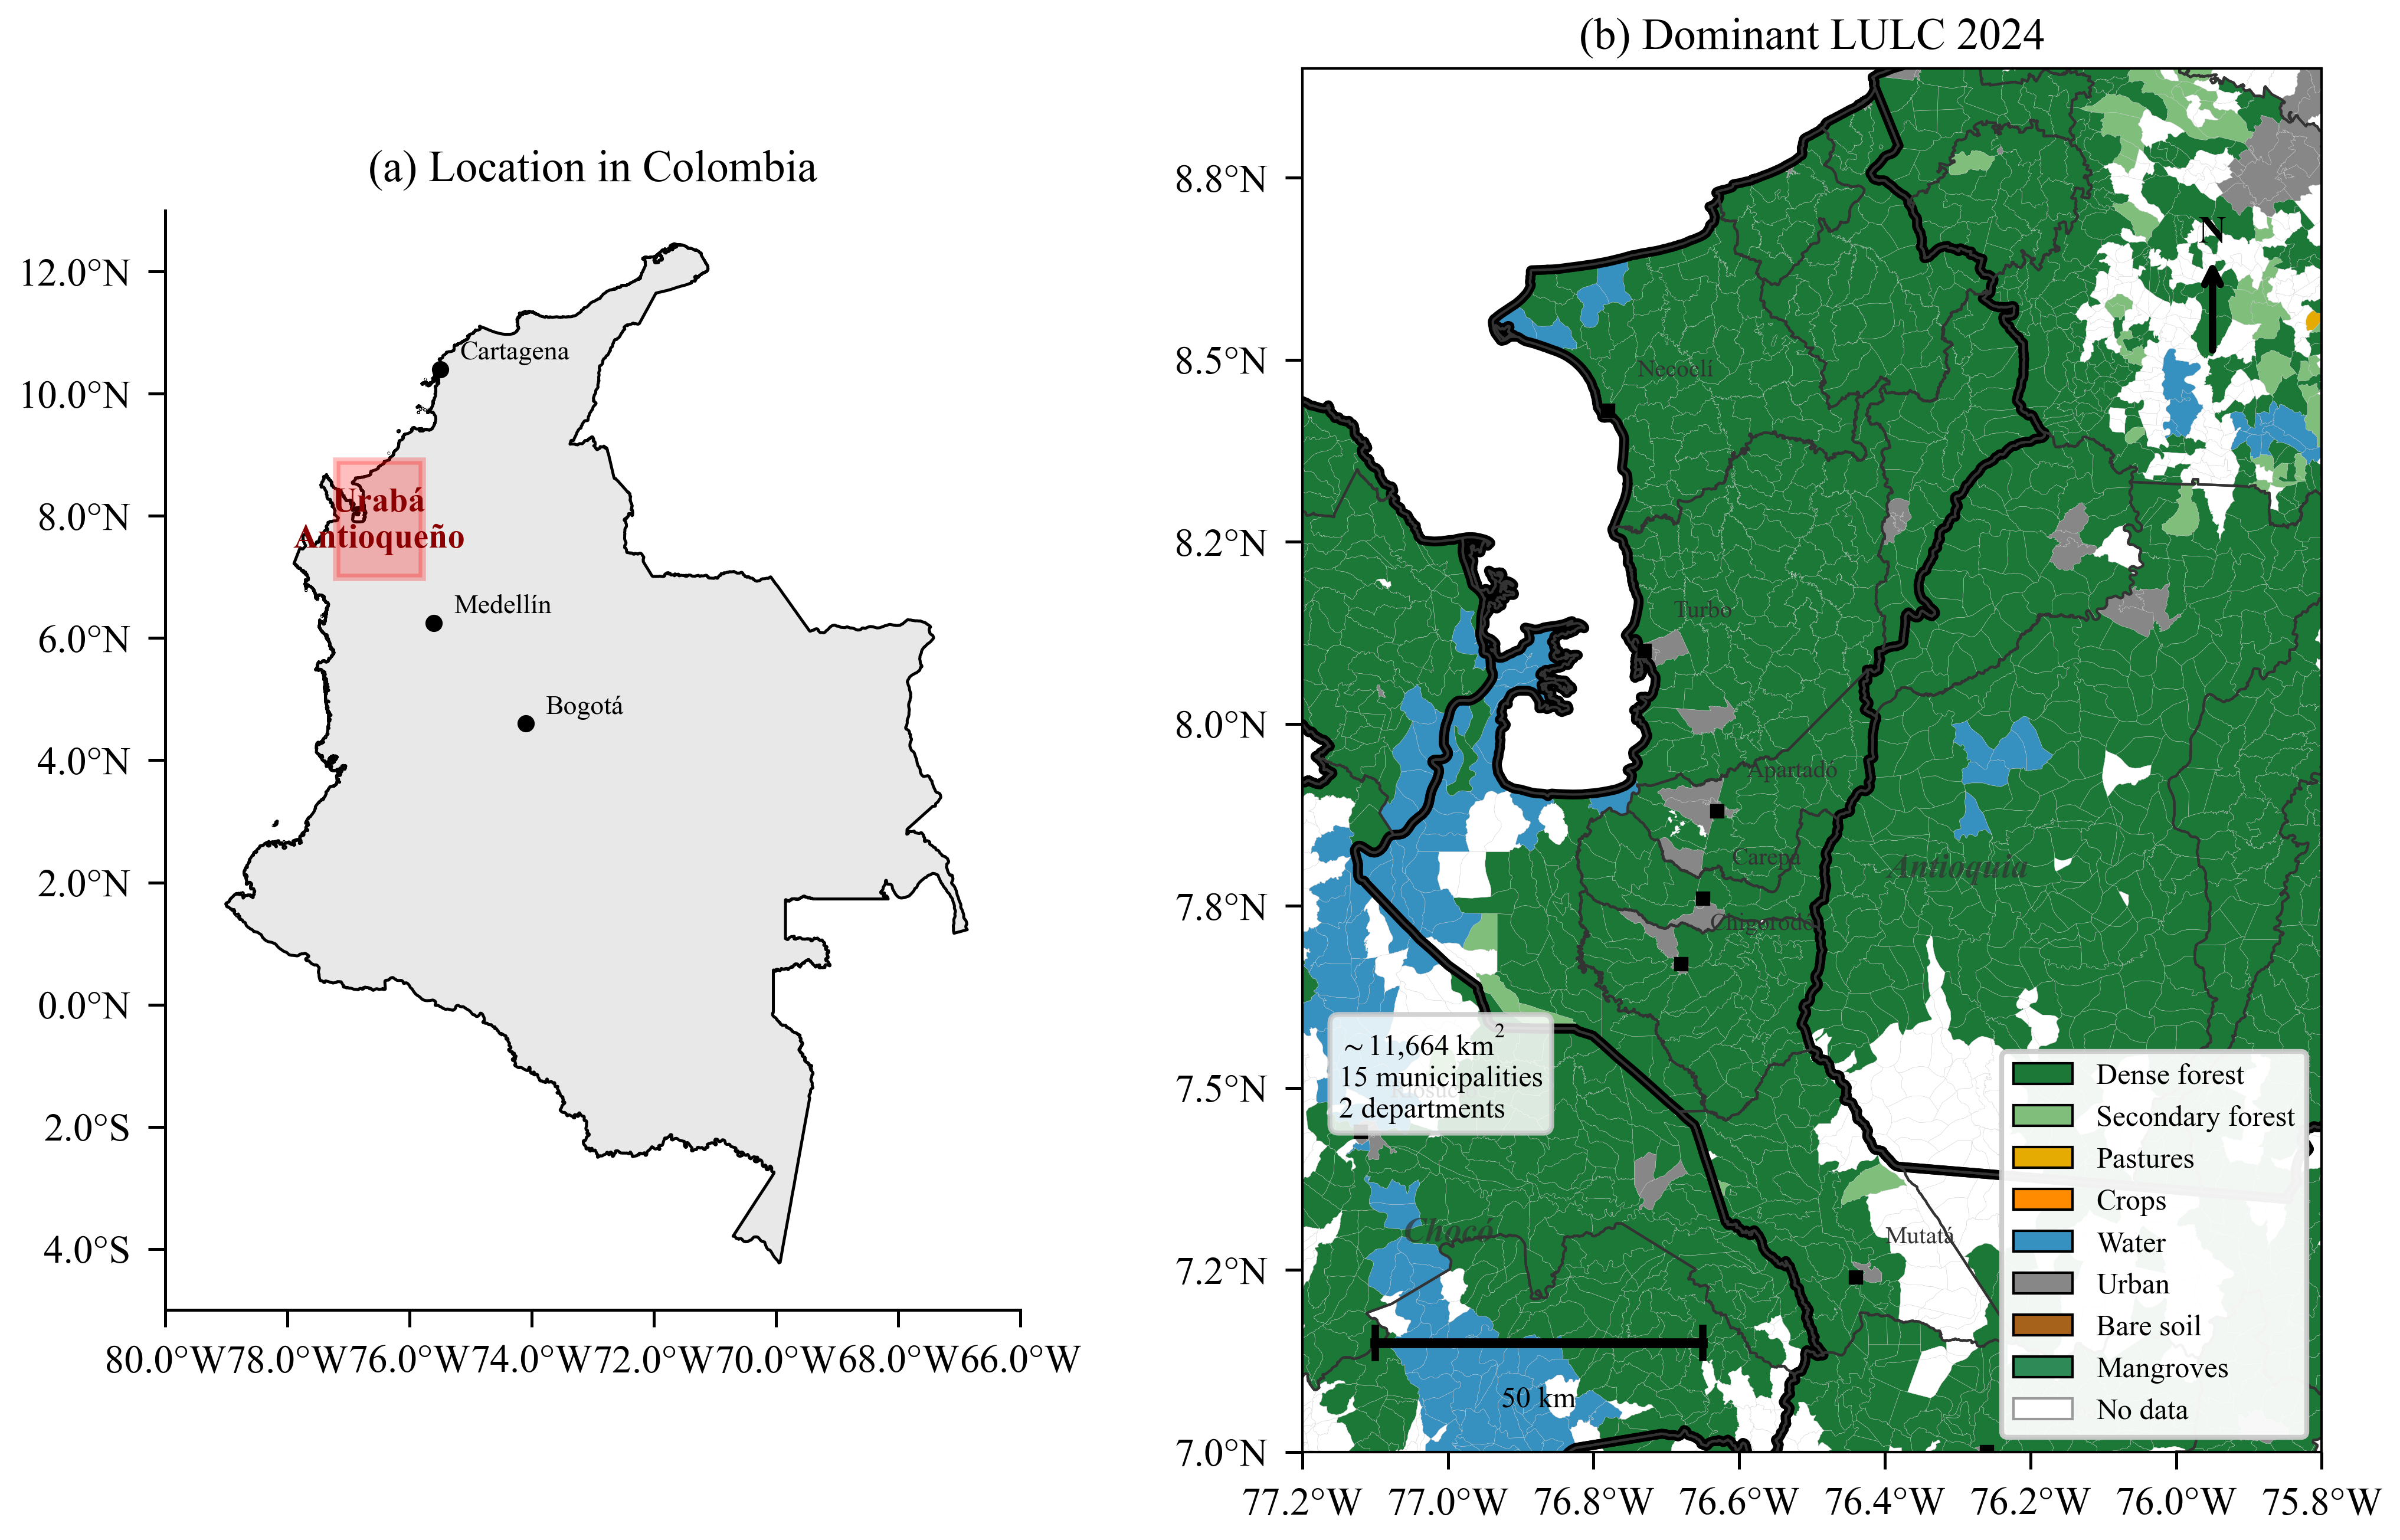
\includegraphics[width=\textwidth]{fig01_study_area_choropleth.png}
\caption{Study area: (a)~Location of Urab\'{a} Antioque\~{n}o in Colombia; (b)~Veredal-level choropleth of dominant LULC class (2024) with municipal boundaries (thin gray lines) and departmental boundaries (thick black lines). The study area encompasses 15 municipalities (${\sim}$11,000~km$^2$) across two departments (Antioquia and Choc\'{o}), bordering the Gulf of Urab\'{a} and the Dari\'{e}n Gap.\label{fig:study_area}}
\end{figure}

\subsection{Socioeconomic and Conflict Context}

Urab\'{a} has been historically one of Colombia's most conflict-affected regions, with a distinct trajectory from the FARC-dominated narrative of southern Colombia. The region was the epicenter of paramilitary consolidation in the 1990s: the AUC under Carlos Casta\~{n}o established territorial control through systematic violence, forced displacement, and land dispossession, particularly targeting banana worker unions and Afro-Colombian communities \citep{GarciaDeLaTorre2011,Uribe2001,GutierrezSanin2014}. Following AUC demobilization (2003--2006), the Clan del Golfo emerged as the dominant successor group, maintaining drug trafficking routes and territorial control \citep{Grajales2011,Grajales2015}.

The 2016 peace agreement designated Urab\'{a} municipalities as PDET territories (Planes de Desarrollo con Enfoque Territorial), prioritized for post-conflict territorial development. Land restitution under Ley 1448 has been particularly contentious, with an estimated 40,000+ hectares subject to restitution claims linked to paramilitary-era dispossession \citep{SanchezGomez2020}. Since 2019, the Dari\'{e}n Gap has become the world's most transited irregular migration corridor, with over 500,000 crossings in 2023 alone, adding new pressures to governance and natural resources.

The region's economy combines formal agroindustry (banana exports generating \$800+ million annually), oil palm cultivation \citep{Castiblanco2013}, extensive cattle ranching, illegal gold mining, and coca cultivation---creating a complex mosaic of legal and illegal land use pressures operating across ecological gradients from coastal mangroves to montane forests.

\subsection{Analysis Periods}

We defined four analysis periods aligned with key political milestones, identical to those used in a parallel study of Colombia's Magdalena Medio to enable cross-regional comparison:

\begin{itemize}
\item \textbf{T1: Pre-agreement (2012--2014):} Havana peace negotiations ongoing; AUC post-demobilization; FARC and Clan del Golfo presence; banana/palm expansion continuing. Representative year: 2013.
\item \textbf{T2: Transition (2015--2017):} Peace agreement signed (November 2016); FARC demobilization; governance vacuums; Clan del Golfo expansion into former FARC areas. Representative year: 2016.
\item \textbf{T3: Early post-agreement (2019--2021):} PDET Urab\'{a} implementation begins; COVID-19 pandemic; migration crisis through Dari\'{e}n; deforestation surge. Representative year: 2020.
\item \textbf{T4: Recent post-agreement (2023--2024):} Petro government's ``Paz Total'' policy; national deforestation reduction efforts; port development in Turbo; continued PDET implementation. Representative year: 2024.
\end{itemize}


%%%%%%%%%%%%%%%%%%%%%%%%%%%%%%%%%%%%%%%%%%
\section{Materials and Methods}
%%%%%%%%%%%%%%%%%%%%%%%%%%%%%%%%%%%%%%%%%%

\subsection{Data Sources}

\subsubsection{Satellite Imagery}

Multi-temporal composites were generated from Landsat~8/9 Collection~2 Level~2 Surface Reflectance (USGS; 30~m; \citealp{Wulder2022}) and Sentinel-2 SR Harmonized (ESA/Copernicus; 10--20~m; \citealp{Drusch2012}) imagery accessed through Google Earth Engine (GEE project: ee-maestria-tesis). Due to the extremely high cloud cover characteristic of the Choc\'{o} bioregion, temporal compositing windows were extended to $\pm$1.5 years around each representative year to ensure sufficient cloud-free pixels. Cloud masking followed sensor-specific protocols: QA\_PIXEL bitwise flags for Landsat and Scene Classification Layer (SCL) bands 3, 8, 9, 10, 11 for Sentinel-2. Surface reflectance scaling factors were applied: multiply(0.0000275).add($-$0.2) for Landsat and multiply(0.0001) for Sentinel-2.

\subsubsection{Mangrove Reference Data}

Mangrove extent was derived from the Global Mangrove Watch (GMW) 2020 baseline dataset \citep{BlancoLibreros2015,Polidoro2010} accessed via GEE (\texttt{projects/global-mangrove-watch/GMW2020}). The GMW provides validated mangrove extent maps at 25~m resolution, used both for training sample generation and for cross-validation of the mangrove LULC class.

\subsubsection{Ancillary Datasets}

Topographic variables (elevation, slope) were derived from SRTM 30~m (USGS). Precipitation data were obtained from CHIRPS Daily v2.0 (${\sim}$5.5~km; \citealp{Funk2015}). Land surface temperature (LST) came from MODIS MOD11A2 v061 (1~km). Population density was sourced from WorldPop (100~m), settlement patterns from GHSL SMOD 2020 (1~km), and permanent water extent from JRC Global Surface Water v1.4 (30~m). Hansen Global Forest Change v1.12 (30~m; through 2024; \citealp{Hansen2013}) provided independent forest loss validation and reference data for training sample generation.

\subsection{LULC Classification}

\subsubsection{Classification Scheme}

We adopted an eight-class LULC scheme reflecting the diverse land covers of Urab\'{a}, including a dedicated mangrove class critical for this coastal region: (1)~Dense forest (canopy cover $>$60\%, humid tropical), (2)~Secondary/fragmented forest (canopy cover 30--60\%, successional), (3)~Pastures/grasslands, (4)~Croplands (banana, plantain, oil palm, coca), (5)~Water bodies (Gulf of Urab\'{a}, R\'{i}o Atrato, wetlands), (6)~Urban/built-up, (7)~Bare soil/mining, and (8)~Mangroves (coastal mangrove forests, estuarine).

\subsubsection{Training Sample Generation}

Reference LULC data were generated through a rule-based approach combining multiple global datasets: (i)~Hansen Global Forest Change v1.12 treecover2000 and loss year for forest/non-forest discrimination (dense forest: treecover2000 $\geq$ 60\% with no loss by target year; secondary forest: treecover2000 30--60\%), (ii)~JRC Global Surface Water for permanent water bodies (occurrence $>$ 50\%), (iii)~GHSL SMOD for urban areas (smod $\geq$ 20), (iv)~Global Mangrove Watch (GMW) 2020 for mangrove training samples---mangroves were assigned the highest priority in the reference map after water to prevent confusion with terrestrial forest classes. Stratified random sampling generated approximately 500 points per class (total ${\sim}$4,000 per period across 8 classes), split 70/30 for training and validation.

\subsubsection{Feature Extraction and Classification}

For each period, pixel-level composites included 12 features: 6 surface reflectance bands (blue, green, red, NIR, SWIR1, SWIR2), 4 spectral indices (NDVI, NDWI, NDBI, NBR), and 2 topographic variables (elevation, slope). Classification used Random Forest \citep[\texttt{ee.Classifier.smileRandomForest};][]{Breiman2001} with 200 trees, minimum leaf population of~5, and bag fraction of 0.632, with tileScale=4 and bestEffort=True to manage computational constraints.

\subsubsection{Post-Processing}

Classified maps were exported as Int8 images to reduce computation chain complexity, water bodies were enforced using JRC Global Surface Water pixels with $>$80\% temporal occurrence, and mangrove extent was cross-referenced with GMW to reduce commission errors in non-coastal areas.

\subsection{Accuracy Assessment}

Classification accuracy was evaluated using error matrices from the 30\% hold-out validation set \citep{Congalton1991,Foody2002}. Following best practices for area estimation under imperfect classification \citep{Olofsson2014,Stehman2019}, we applied stratified area estimators that weight confusion matrix entries by mapped-class proportions ($W_i = A_{\text{map},i} / A_{\text{total}}$) to obtain unbiased area estimates with 95\% confidence intervals. The Kappa coefficient was replaced by quantity disagreement~(QD) and allocation disagreement~(AD) following \citet{Pontius2011} and \citet{Foody2020}. Adjusted overall accuracy, per-class user's and producer's accuracies, and their standard errors were computed using the variance estimators of \citet{Olofsson2014}.

\subsection{Change Detection}

\subsubsection{Transition Matrices}

Three transition matrices were computed for sequential period pairs (T1$\rightarrow$T2, T2$\rightarrow$T3, T3$\rightarrow$T4). Areas (ha) for each from-to class combination were calculated via pixel counting, yielding persistence, gross gains, gross losses, net change, and annual rates for each class. Annual rates were calculated as: $r = (\Delta A / A_{t_1}) / \Delta t \times 100$ \citep{Puyravaud2003}.

\subsubsection{Hansen GFC Cross-Validation}

Forest loss detected through our classification was cross-validated against Hansen GFC v1.12 loss year data, aggregated by analysis period.

\subsection{Spatial Statistical Analysis}

\subsubsection{Spatial Autocorrelation}

Moran's~$I$ global statistic \citep{Moran1950,Anselin1995} was computed to test for spatial autocorrelation in deforestation rates across 1$\times$1~km grid cells, using distance-based Queen contiguity weights.

\subsubsection{Hotspot Analysis}

Getis-Ord Gi* local statistics \citep{Getis1992} identified statistically significant hotspots (high deforestation clustering) and coldspots (low deforestation clustering) at 90\%, 95\%, and 99\% confidence levels.

\subsubsection{Kernel Density Estimation}

Gaussian kernel density estimation provided continuous surface representations of deforestation intensity.

\subsection{Ecosystem Service Assessment}

\subsubsection{Carbon Storage}

Carbon stocks (Mg~C~ha$^{-1}$) were estimated for each LULC class using IPCC Tier~2 values calibrated for the Choc\'{o} bioregion \citep{Alvarez2012,Phillips2019,IDEAM2018} across four pools: aboveground biomass ($C_\text{above}$), belowground biomass ($C_\text{below}$), soil organic carbon ($C_\text{soil}$), and dead organic matter ($C_\text{dead}$). Values per class (total $\pm$ SE Mg~C~ha$^{-1}$): dense forest ($281 \pm 27$), secondary forest ($146 \pm 17$), pastures ($44 \pm 8$), crops ($54 \pm 10$), water~(0), urban ($20 \pm 5$), bare soil ($15 \pm 4$), and mangroves ($247 \pm 45$). Mangrove carbon values follow \citet{Donato2011} and \citet{Twilley2018}, with exceptionally high soil carbon ($120 \pm 30$~Mg~C~ha$^{-1}$) reflecting anaerobic preservation in coastal sediments (``blue carbon''). Total carbon per period was computed using Olofsson-adjusted areas, with uncertainty propagated as $\text{Var}(C_i) = c_i^2 \, \text{Var}(A_i) + A_i^2 \, \text{Var}(c_i) + \text{Var}(A_i) \, \text{Var}(c_i)$ for each class~$i$.

\subsubsection{Water Yield}

Seasonal water yield was estimated as annual precipitation (CHIRPS) minus evapotranspiration derived from MODIS MOD16A2 v061, adjusted by LULC-specific crop coefficients ($K_c$) following FAO~56: dense forest (1.0), secondary forest (0.85), pastures (0.60), croplands (0.70), water bodies (1.20), urban (0.30), bare soil (0.15), and mangroves (0.90). Baseflow recharge was estimated using LULC-dependent infiltration coefficients.

\subsubsection{Habitat Quality}

Habitat quality was modeled following the InVEST framework \citep{Sharp2020}: habitat suitability scores (0--1) were assigned per LULC class (dense forest: 1.0, secondary forest: 0.7, pastures: 0.2, croplands: 0.1, water: 0.5, urban: 0.0, bare soil: 0.0, mangroves: 0.9), and threat layers were constructed from proximity to agriculture/pastures and urban areas using exponential decay functions.

\subsection{Driver Analysis}

\subsubsection{Variable Preparation}

Nine spatially explicit driver variables were prepared in GEE at 1~km resolution: elevation, slope, distance to rivers, distance to roads, distance to urban centers, population density (WorldPop 2020), mean annual precipitation (CHIRPS 2012--2024), mean LST (MODIS 2012--2024), and clay content (SoilGrids). The dependent variable was the deforestation rate (\%~yr$^{-1}$) for the post-agreement period. Variance Inflation Factors (VIF) were computed to assess multicollinearity (threshold: VIF~$<$~10).

\subsubsection{OLS and GWR Regression}

An Ordinary Least Squares (OLS) model was fitted as a baseline. GWR with adaptive bisquare kernel \citep{Fotheringham2002} was fitted to capture spatial non-stationarity, with bandwidth optimized via AICc minimization. Model comparison used $R^2$, AICc, and residual analysis. We report the effective number of parameters (ENP) and the ENP/$n$ ratio as indicators of model complexity, and present bandwidth sensitivity analysis to assess the robustness of spatial non-stationarity.

\subsection{Future Scenario Modeling}

\subsubsection{CA-Markov Model}

Markov chain transition probability matrices \citep{Halmy2015} were calibrated from stratified random sample points across the 2020--2024 LULC transitions. Ecological constraints were applied to correct implausible transitions. The corrected model was projected for 2030 and 2040 under three scenarios:

\begin{itemize}
\item \textbf{Business-as-usual (BAU):} Current transition rates persist; banana/palm expansion continues; Clan del Golfo territorial presence maintained.
\item \textbf{Conservation:} Deforestation rates reduced by 50\%; Kat\'{i}os NP buffer zone enforced; mangrove restoration along Gulf coast; recovery rates increased by 30\%.
\item \textbf{PDET Urab\'{a}:} Deforestation rates reduced by 30\%; land restitution programs implemented; sustainable rural development with agricultural diversification increased by 20\%.
\end{itemize}

\subsection{Climate Analysis}

Annual precipitation (CHIRPS) and LST (MODIS MOD11A2) time series for 2012--2024 were analyzed for trends using the Mann-Kendall test and Sen's slope estimator. Standardized Precipitation Index (SPI) was calculated to identify drought events.


%%%%%%%%%%%%%%%%%%%%%%%%%%%%%%%%%%%%%%%%%%
\section{Results}
%%%%%%%%%%%%%%%%%%%%%%%%%%%%%%%%%%%%%%%%%%

\subsection{Classification Accuracy}

After applying \citet{Olofsson2014} stratified estimators to the 8-class system, adjusted overall accuracies were 66.5\%~(T1: 2013), 71.0\%~(T2: 2016), 66.5\%~(T3: 2020), and 71.9\%~(T4: 2024) (Table~\ref{tab:accuracy}). Quantity disagreement ranged from 0.055~(T3) to 0.090~(T1), while allocation disagreement ranged from 0.218~(T4) to 0.280~(T3). Adjusted user's accuracy for dense forest ranged from 44.0\% to 56.2\%, while the mangrove class achieved 82.5--93.3\% UA, reflecting the distinct spectral signature of coastal mangrove forests. The moderate overall accuracies reflect the inherent challenge of discriminating eight LULC classes in the exceptionally cloud-prone Choc\'{o} bioregion; the Olofsson framework explicitly accounts for this uncertainty in all area estimates.

Feature importance rankings (Figure~S1) consistently identified SWIR1, elevation, SWIR2, and NDWI as the top-ranked variables across all periods, with NDWI gaining particular importance for discriminating mangroves from terrestrial forest classes.

\begin{table}[!ht]
\caption{Classification accuracy assessment results.\label{tab:accuracy}}
\begin{threeparttable}
\begin{tabular*}{\textwidth}{@{\extracolsep{\fill}}lccccccc@{\extracolsep{\fill}}}
\toprule
Period & Year & Images & Training & Validation & OA$_\text{adj}$ (\%) & QD & AD \\
\midrule
T1 & 2013 & 76 & 1,277 & 513 & 66.5 & 0.090 & 0.246 \\
T2 & 2016 & 125 & 1,243 & 556 & 71.0 & 0.063 & 0.227 \\
T3 & 2020 & 823 & 1,292 & 508 & 66.5 & 0.055 & 0.280 \\
T4 & 2024 & 758 & 1,309 & 491 & 71.9 & 0.063 & 0.218 \\
\bottomrule
\end{tabular*}
\begin{tablenotes}
\item Source: OA$_\text{adj}$: Olofsson-adjusted overall accuracy \citep{Olofsson2014}; QD: quantity disagreement; AD: allocation disagreement \citep{Pontius2011}. Eight-class system including mangroves.
\end{tablenotes}
\end{threeparttable}
\end{table}

\subsection{LULC Maps and Area Changes}

The four classified LULC maps (Figures~\ref{fig:lulc_maps} and~\ref{fig:composition}) reveal a landscape undergoing substantial transformation over the study period (Table~\ref{tab:areas}). Dense forest area was estimated at \num{740642}~ha in 2013~(T1), declining sharply to \num{449476}~ha in 2024~(T4)---a loss of \num{291166}~ha ($-$39.3\%). Secondary forest showed an increasing trend, expanding from \num{510575}~ha~(T1) to \num{657114}~ha~(T4), likely reflecting partial recovery of previously deforested areas. Estimated total forest cover (dense~$+$~secondary~$+$~mangroves) declined from ${\sim}$\num{1330000}~ha in 2013 to ${\sim}$\num{1234400}~ha in 2024, an estimated net loss of ${\sim}$7.2\%.

Mangrove extent was estimated at \num{78770}~ha~(T1), increasing to \num{141736}~ha at T3 before declining to \num{127815}~ha~(T4), concentrated along the Gulf of Urab\'{a} coast and the R\'{i}o Atrato estuary. Pastures expanded substantially from \num{1026478}~ha (2013) to \num{1292644}~ha (2024), confirming cattle ranching as the primary land use replacing forest. The cropland class (banana, plantain, oil palm) was not detected as a separate class in any period, likely due to spectral confusion with pastures and secondary vegetation at 30~m resolution.

\begin{figure}[!ht]
\centering
\includegraphics[width=\textwidth]{fig02_lulc_choropleth_4panel.png}
\caption{Veredal-level LULC choropleth maps for four periods: (a)~T1 (2013), (b)~T2 (2016), (c)~T3 (2020), (d)~T4 (2024). Each vereda is colored by dominant LULC class. Municipal boundaries shown as thin gray lines, departmental boundaries as thick black lines. Eight-class palette including mangroves (sea green) along the Gulf coast.\label{fig:lulc_maps}}
\end{figure}

\begin{figure}[!ht]
\centering
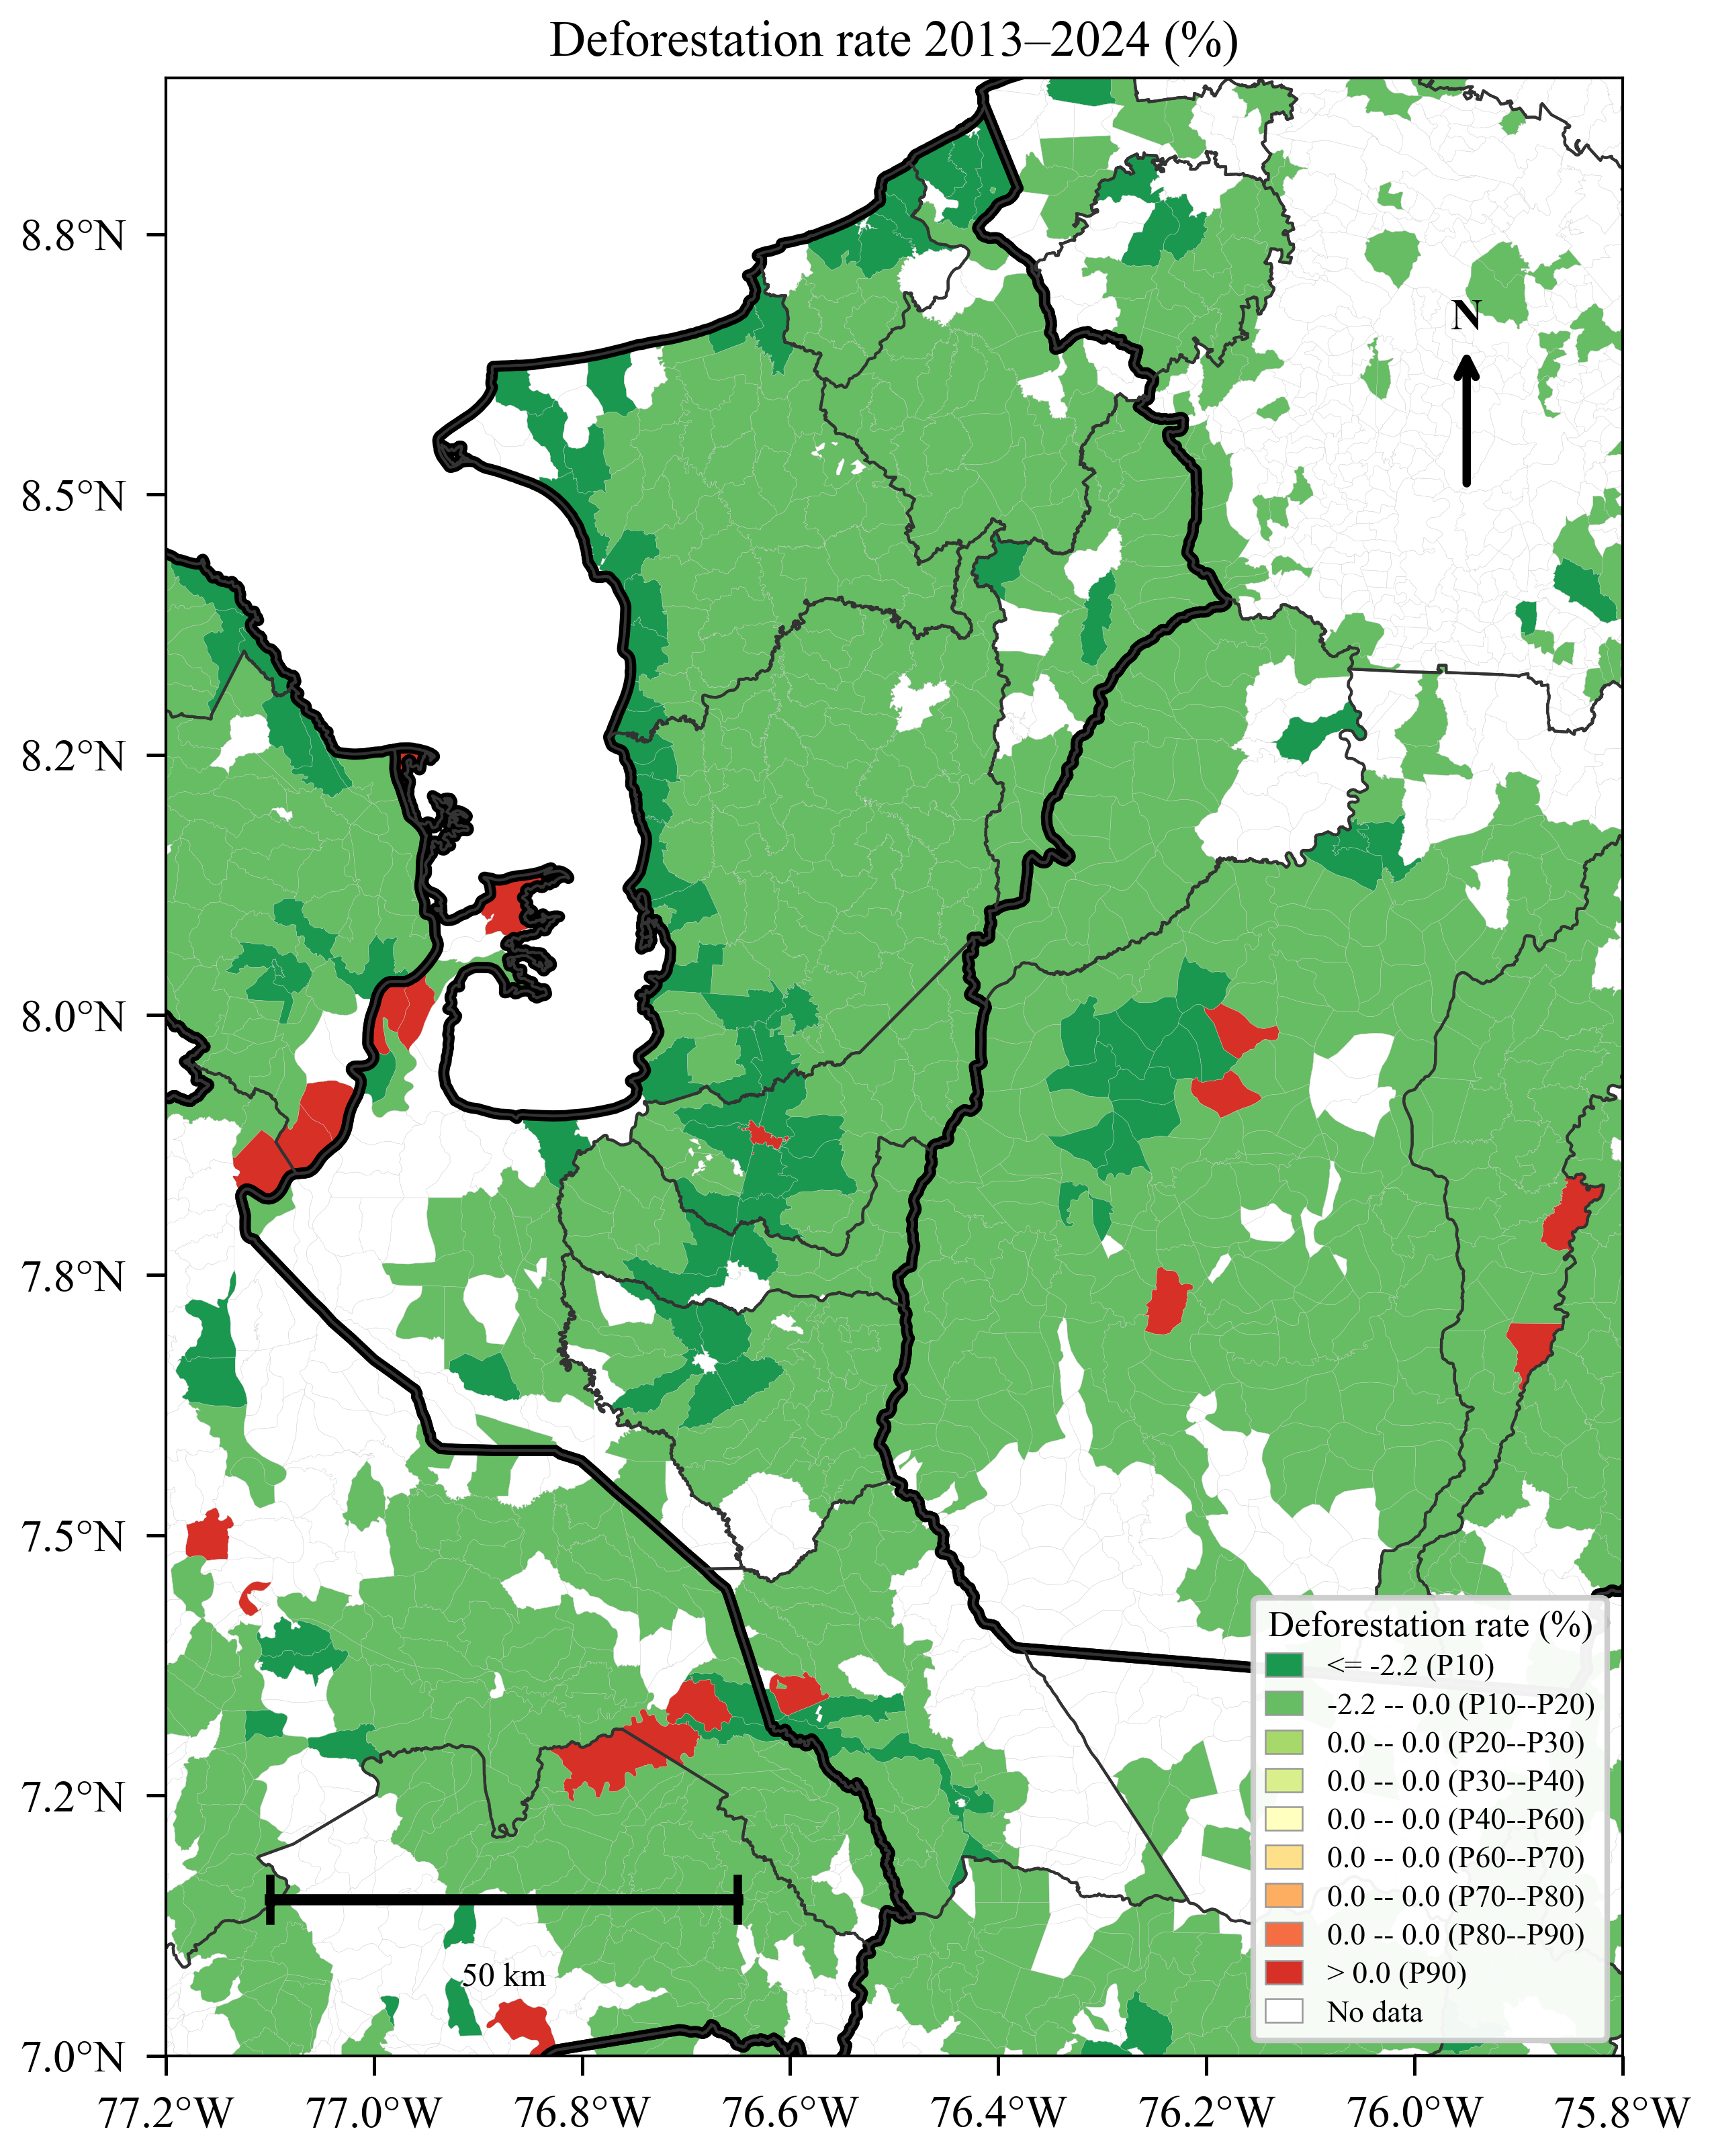
\includegraphics[width=\textwidth]{fig03_deforestation_choropleth.png}
\caption{Veredal-level deforestation intensity choropleth (2013--2024). Veredas colored by deforestation rate (\%) using percentile-based 9-class bins (RdYlGn divergent scale). The Dari\'{e}n frontier and southern montane areas show highest deforestation intensity.\label{fig:forest_change}}
\end{figure}

\begin{figure}[!ht]
\centering
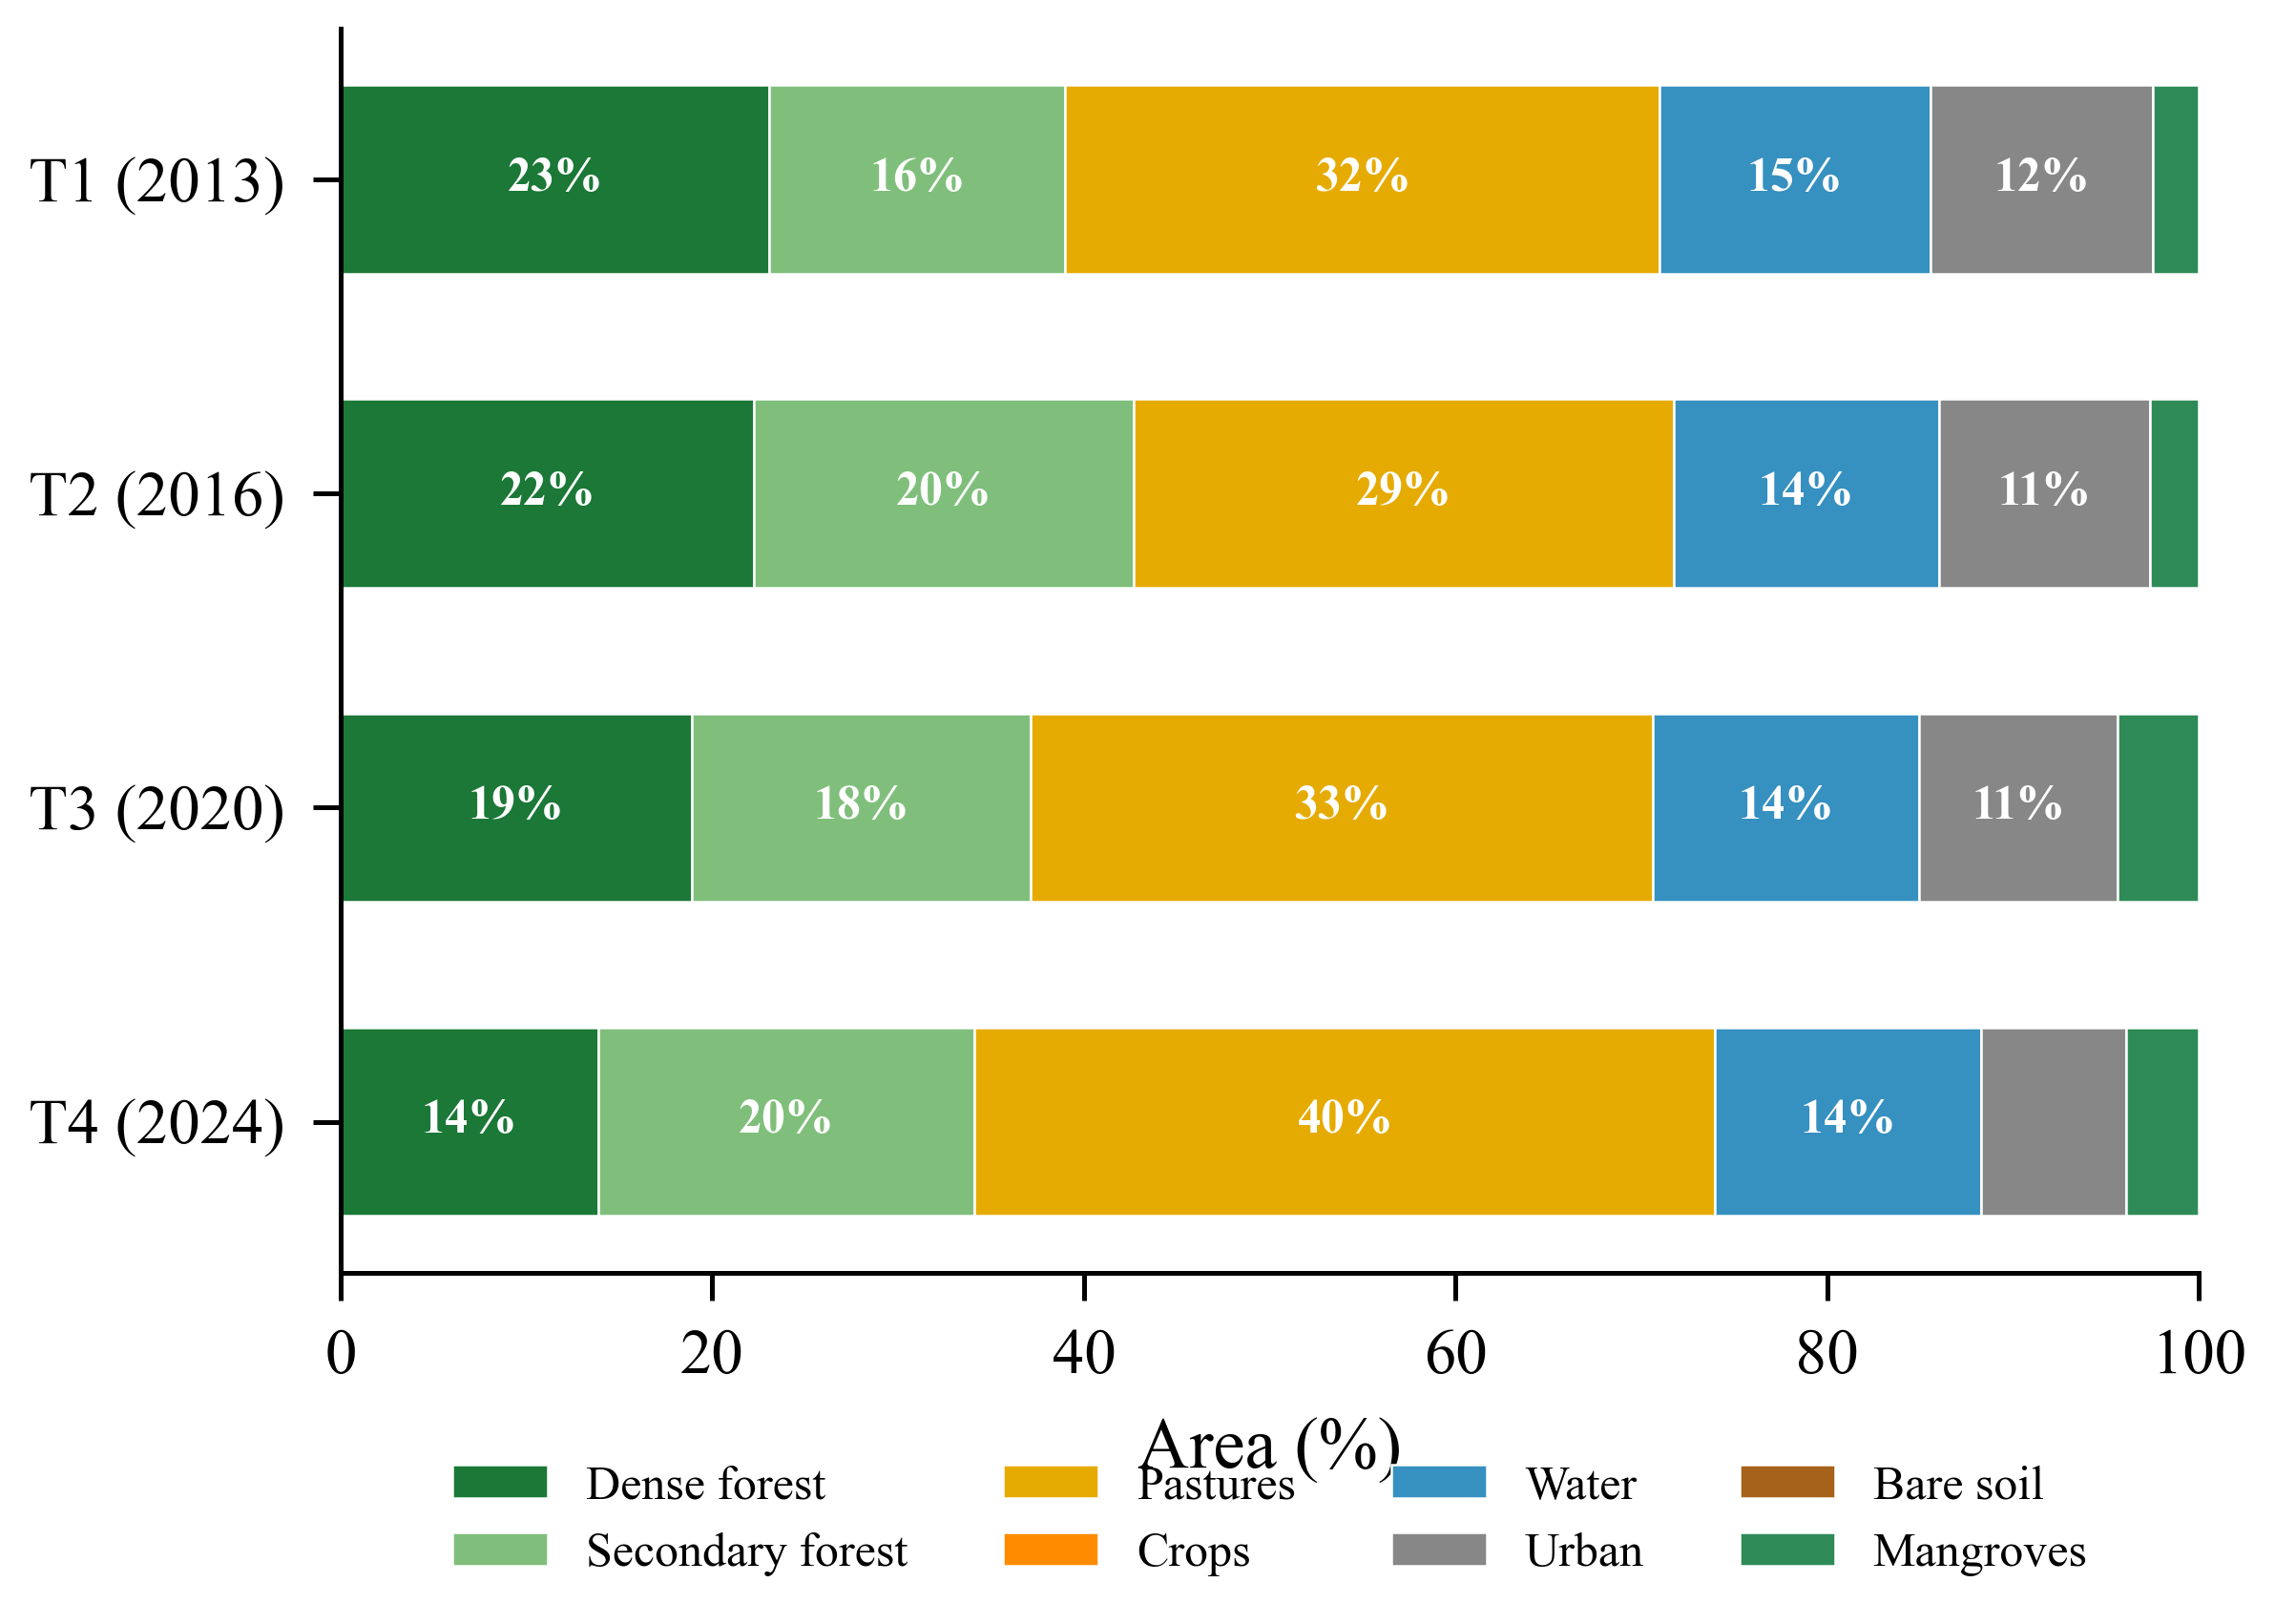
\includegraphics[width=0.7\textwidth]{fig04a_lulc_composition.pdf}
\caption{LULC area composition (\%) for four periods shown as 100\% stacked bar chart, with forest trend (dense + secondary + mangrove) and 95\% Olofsson confidence interval bands.\label{fig:composition}}
\end{figure}

\begin{table}[!ht]
\caption{LULC class areas ($\times 10^3$~ha) by period.\label{tab:areas}}
\begin{threeparttable}
\begin{tabular*}{\textwidth}{@{\extracolsep{\fill}}lcccc@{\extracolsep{\fill}}}
\toprule
Class & T1 (2013) & T2 (2016) & T3 (2020) & T4 (2024) \\
\midrule
Dense forest     & 740.6 & 720.1 & 612.9 & 449.5 \\
Secondary forest & 510.6 & 662.3 & 591.6 & 657.1 \\
Pastures         & 1,026.5 & 941.4 & 1,086.2 & 1,292.6 \\
Crops            & 0 & 0 & 0 & 0 \\
Water            & 467.3 & 463.2 & 464.6 & 464.1 \\
Urban            & 385.0 & 366.8 & 346.5 & 252.4 \\
Bare soil        & 0 & 0 & 0 & 0 \\
Mangroves        & 78.8 & 85.8 & 141.7 & 127.8 \\
\bottomrule
\end{tabular*}
\begin{tablenotes}
\item Source: Areas from pixel-counted classification. Olofsson-adjusted confidence intervals are available in the supplementary materials. Water includes Gulf of Urab\'{a} (deterministic from JRC mask). Mangrove class validated against Global Mangrove Watch. Cropland class not distinguished from pastures at 30~m resolution.
\end{tablenotes}
\end{threeparttable}
\end{table}

\subsection{Transition Matrices and Deforestation Rates}

Transition matrices (Figure~\ref{fig:transitions}) revealed that forest-to-pasture conversion was the dominant land use transition across all periods.

\textbf{T1$\rightarrow$T2 (2013--2016):} The pre-agreement to transition period saw \num{91363}~ha of dense forest convert to pastures, alongside \num{118987}~ha converting to secondary forest. Dense forest experienced a net loss of \num{24176}~ha ($-$1.1\%~yr$^{-1}$).

\textbf{T2$\rightarrow$T3 (2016--2020):} Accelerating deforestation was observed, with \num{174886}~ha of dense forest converting to pastures and \num{124709}~ha to secondary forest. Dense forest experienced a net loss of \num{107169}~ha ($-$4.0\%~yr$^{-1}$), nearly quadrupling the T1$\rightarrow$T2 annual rate.

\textbf{T3$\rightarrow$T4 (2020--2024):} The most recent period showed \num{331960}~ha of dense forest converting to pastures---nearly double the previous period. Dense forest experienced a net loss of \num{163448}~ha ($-$7.8\%~yr$^{-1}$). Mangrove area declined by \num{13921}~ha ($-$2.6\%~yr$^{-1}$), with \num{52396}~ha of mangroves converting to pastures partly offset by gains from other classes.

Hansen GFC v1.12 cross-validation confirmed forest loss trends (Figure~\ref{fig:deforestation}B): \num{26279}~ha (T1), \num{37434}~ha (T2), \num{29211}~ha (T3), and \num{18008}~ha (T4).

\begin{figure}[!ht]
\centering
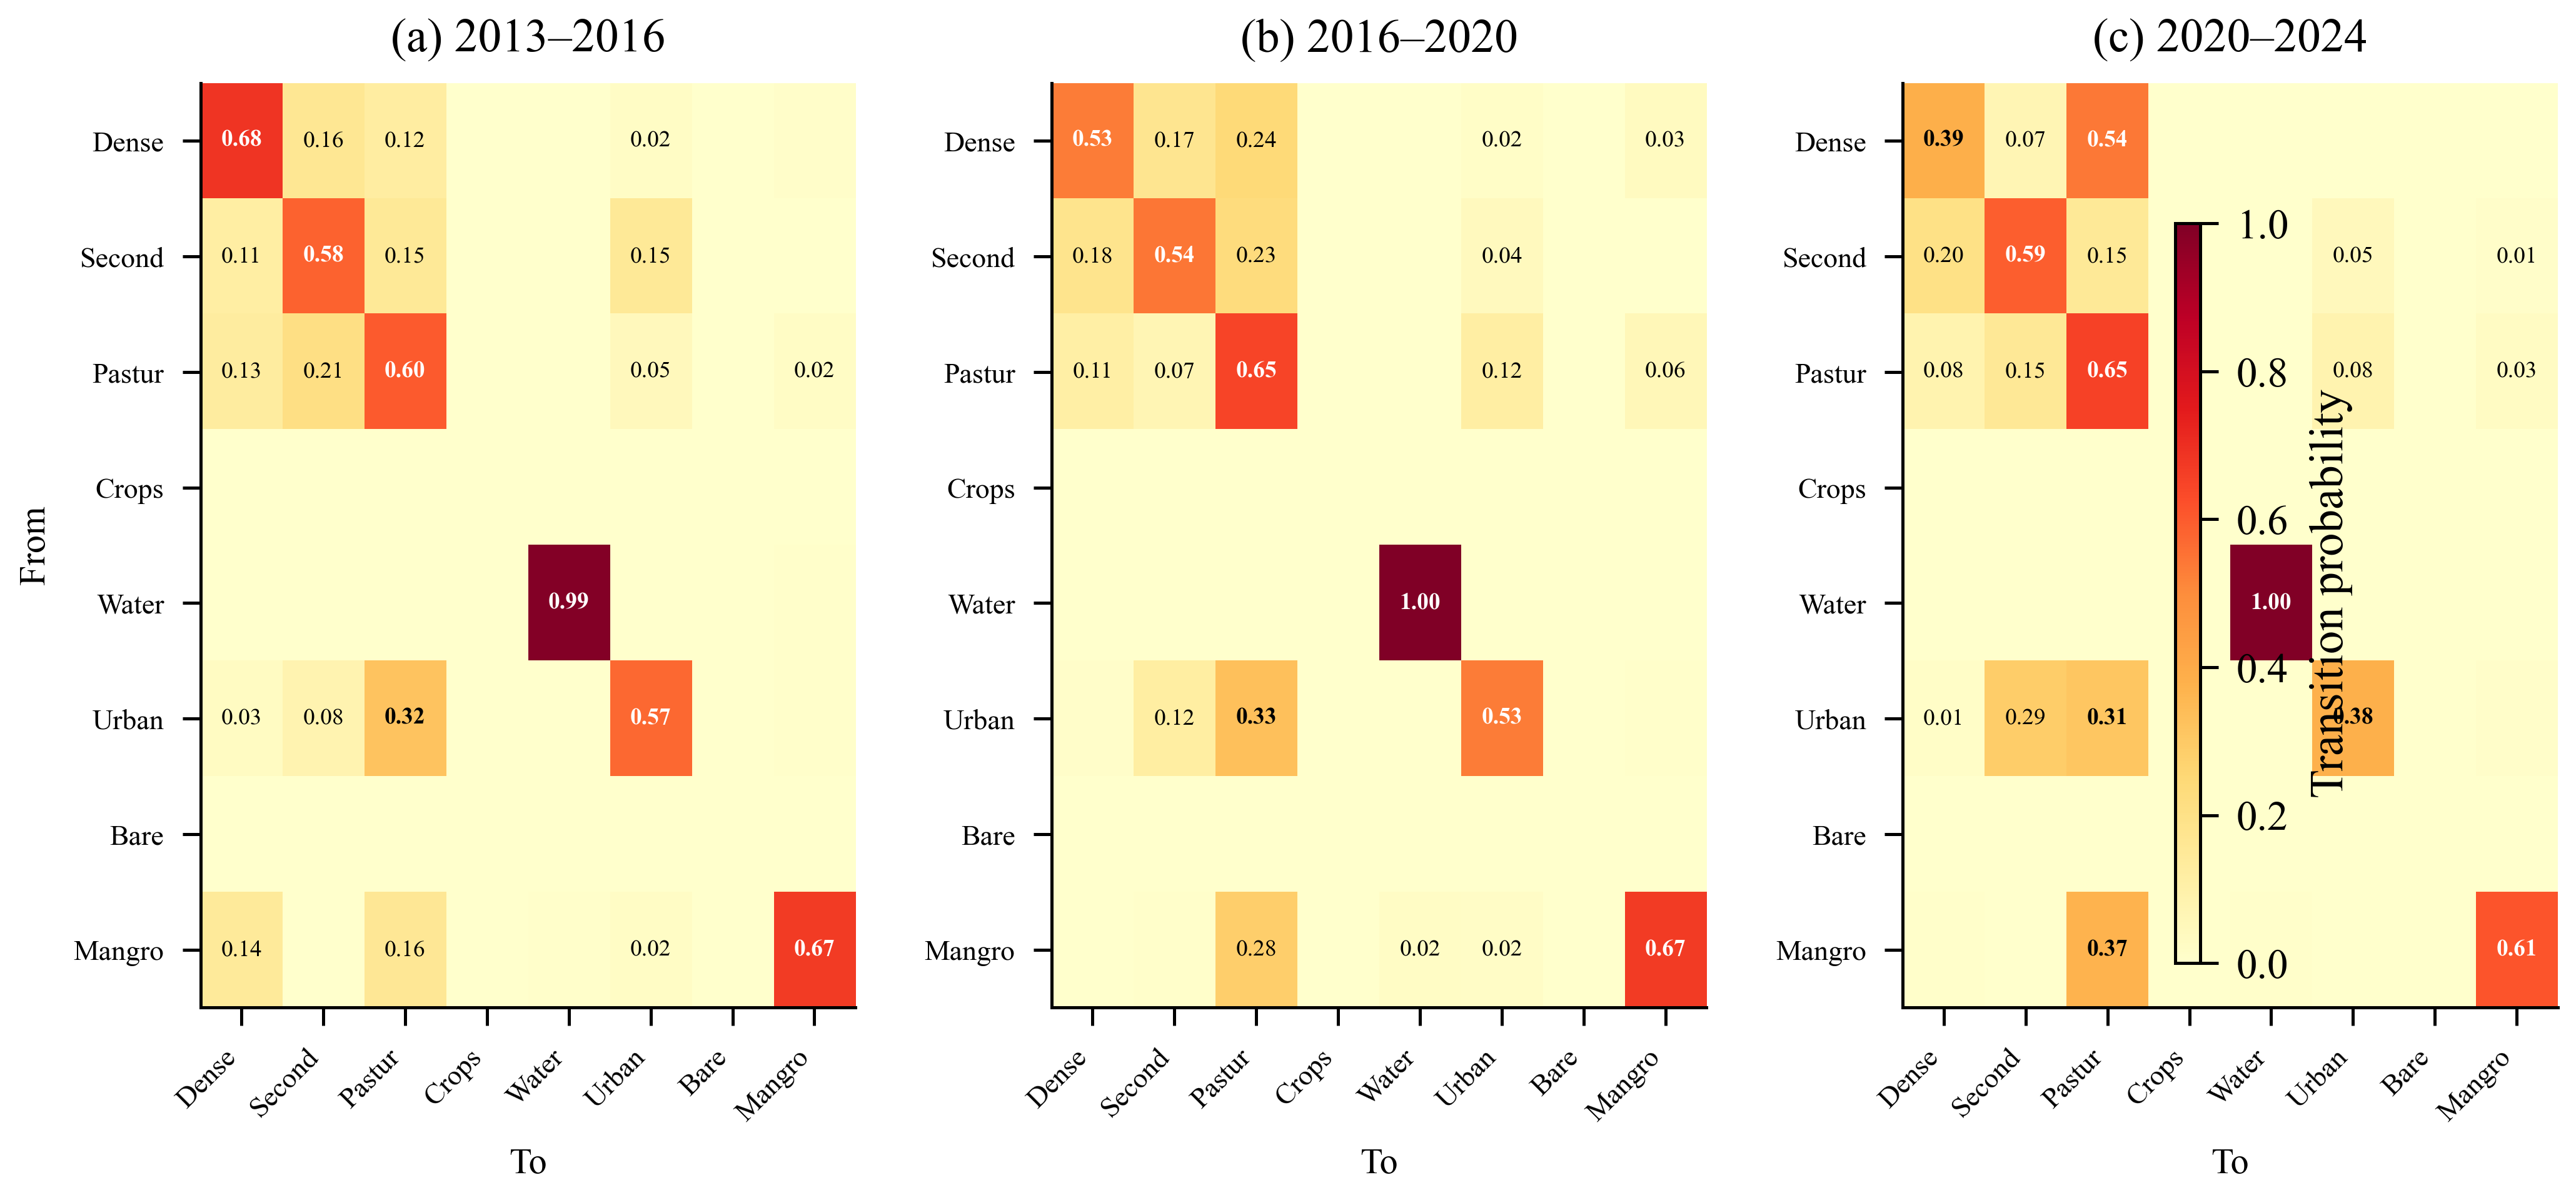
\includegraphics[width=0.7\textwidth]{fig05_transition_matrices.pdf}
\caption{Transition probability matrices (8$\times$8) for three periods: (a)~2013--2016, (b)~2016--2020, (c)~2020--2024. Values represent the proportion of class area at $t_1$ transitioning to each class at $t_2$. The mangrove class shows high persistence but notable transitions to water (erosion) and pastures (conversion).\label{fig:transitions}}
\end{figure}

\begin{figure}[!ht]
\centering
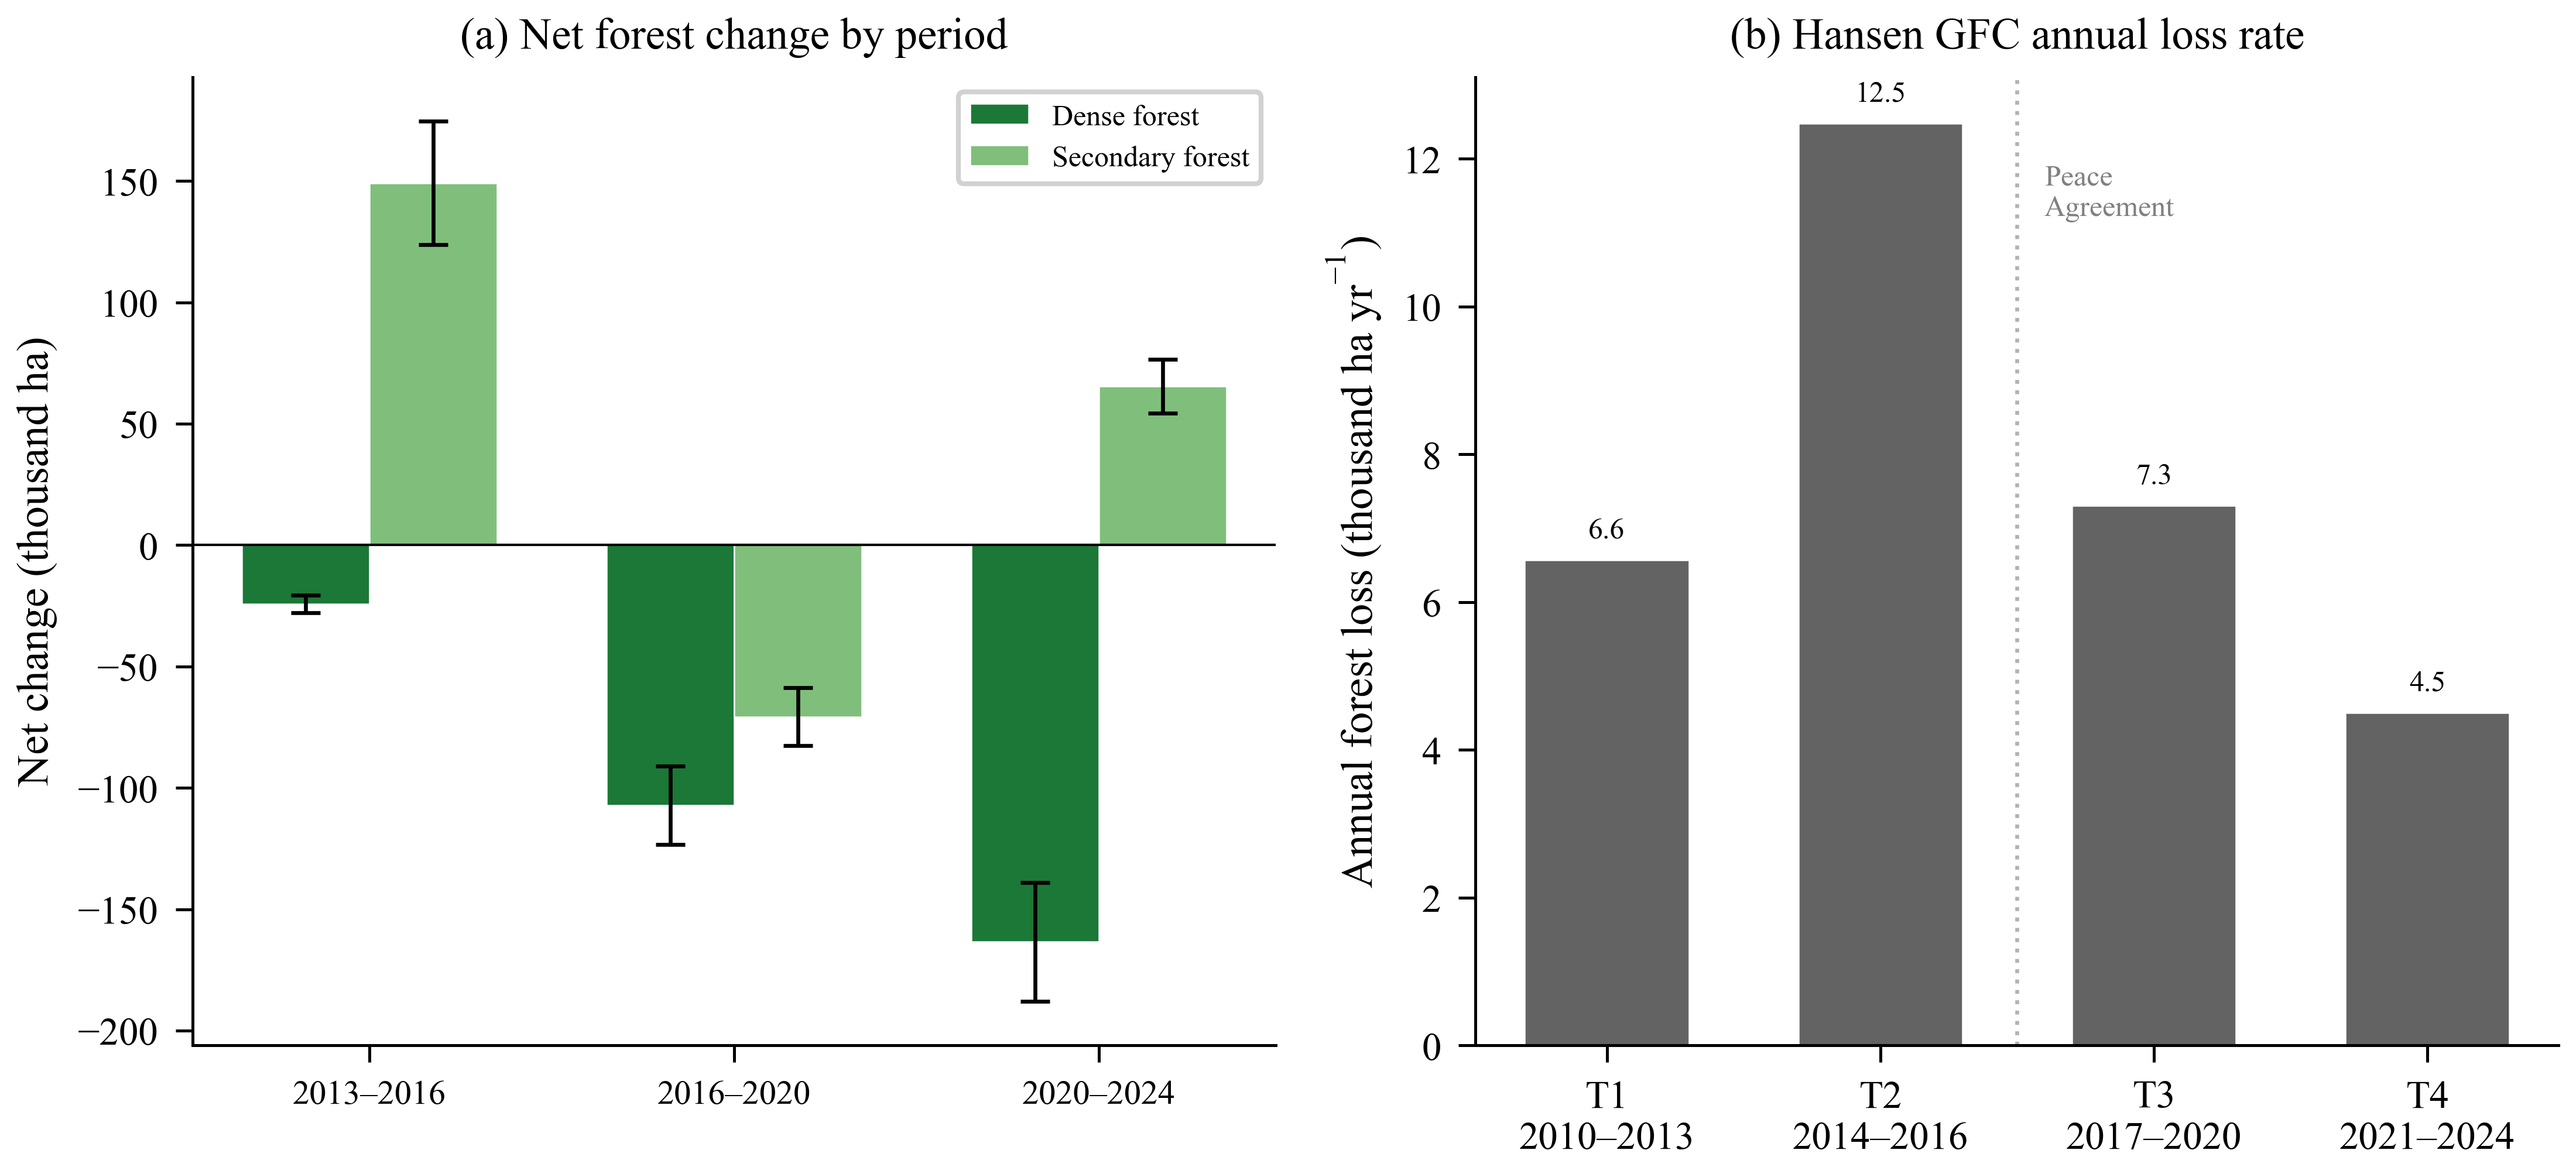
\includegraphics[width=0.7\textwidth]{fig06_deforestation_rates.pdf}
\caption{(A)~Net forest change by period for dense forest, secondary forest, and mangroves with 95\% confidence intervals. (B)~Hansen GFC annual forest loss rate by period.\label{fig:deforestation}}
\end{figure}

\subsection{Spatial Patterns and Hotspots}

Moran's~$I$ global statistic for deforestation rates was 0.010 ($p = 1.0$), indicating weak and non-significant global spatial autocorrelation. Despite the lack of global clustering, the Getis-Ord Gi* local analysis (Figure~\ref{fig:hotspots}) identified 285 statistically significant deforestation hotspot cells at the 99\% confidence level (Z-scores up to 6.30) and 302 significant coldspot cells at 99\% confidence. This divergence between global and local statistics---consistent with spatially heterogeneous patterns---indicates that deforestation is highly concentrated in specific areas rather than uniformly distributed. Hotspots concentrated along the Dari\'{e}n frontier (Acand\'{i}, Ungu\'{i}a), the southern montane zone (Mutat\'{a}, Dabeiba), and areas of recent cattle expansion in the northern coast, while coldspots corresponded to the eje bananero and stable water/urban areas.

\begin{figure}[!ht]
\centering
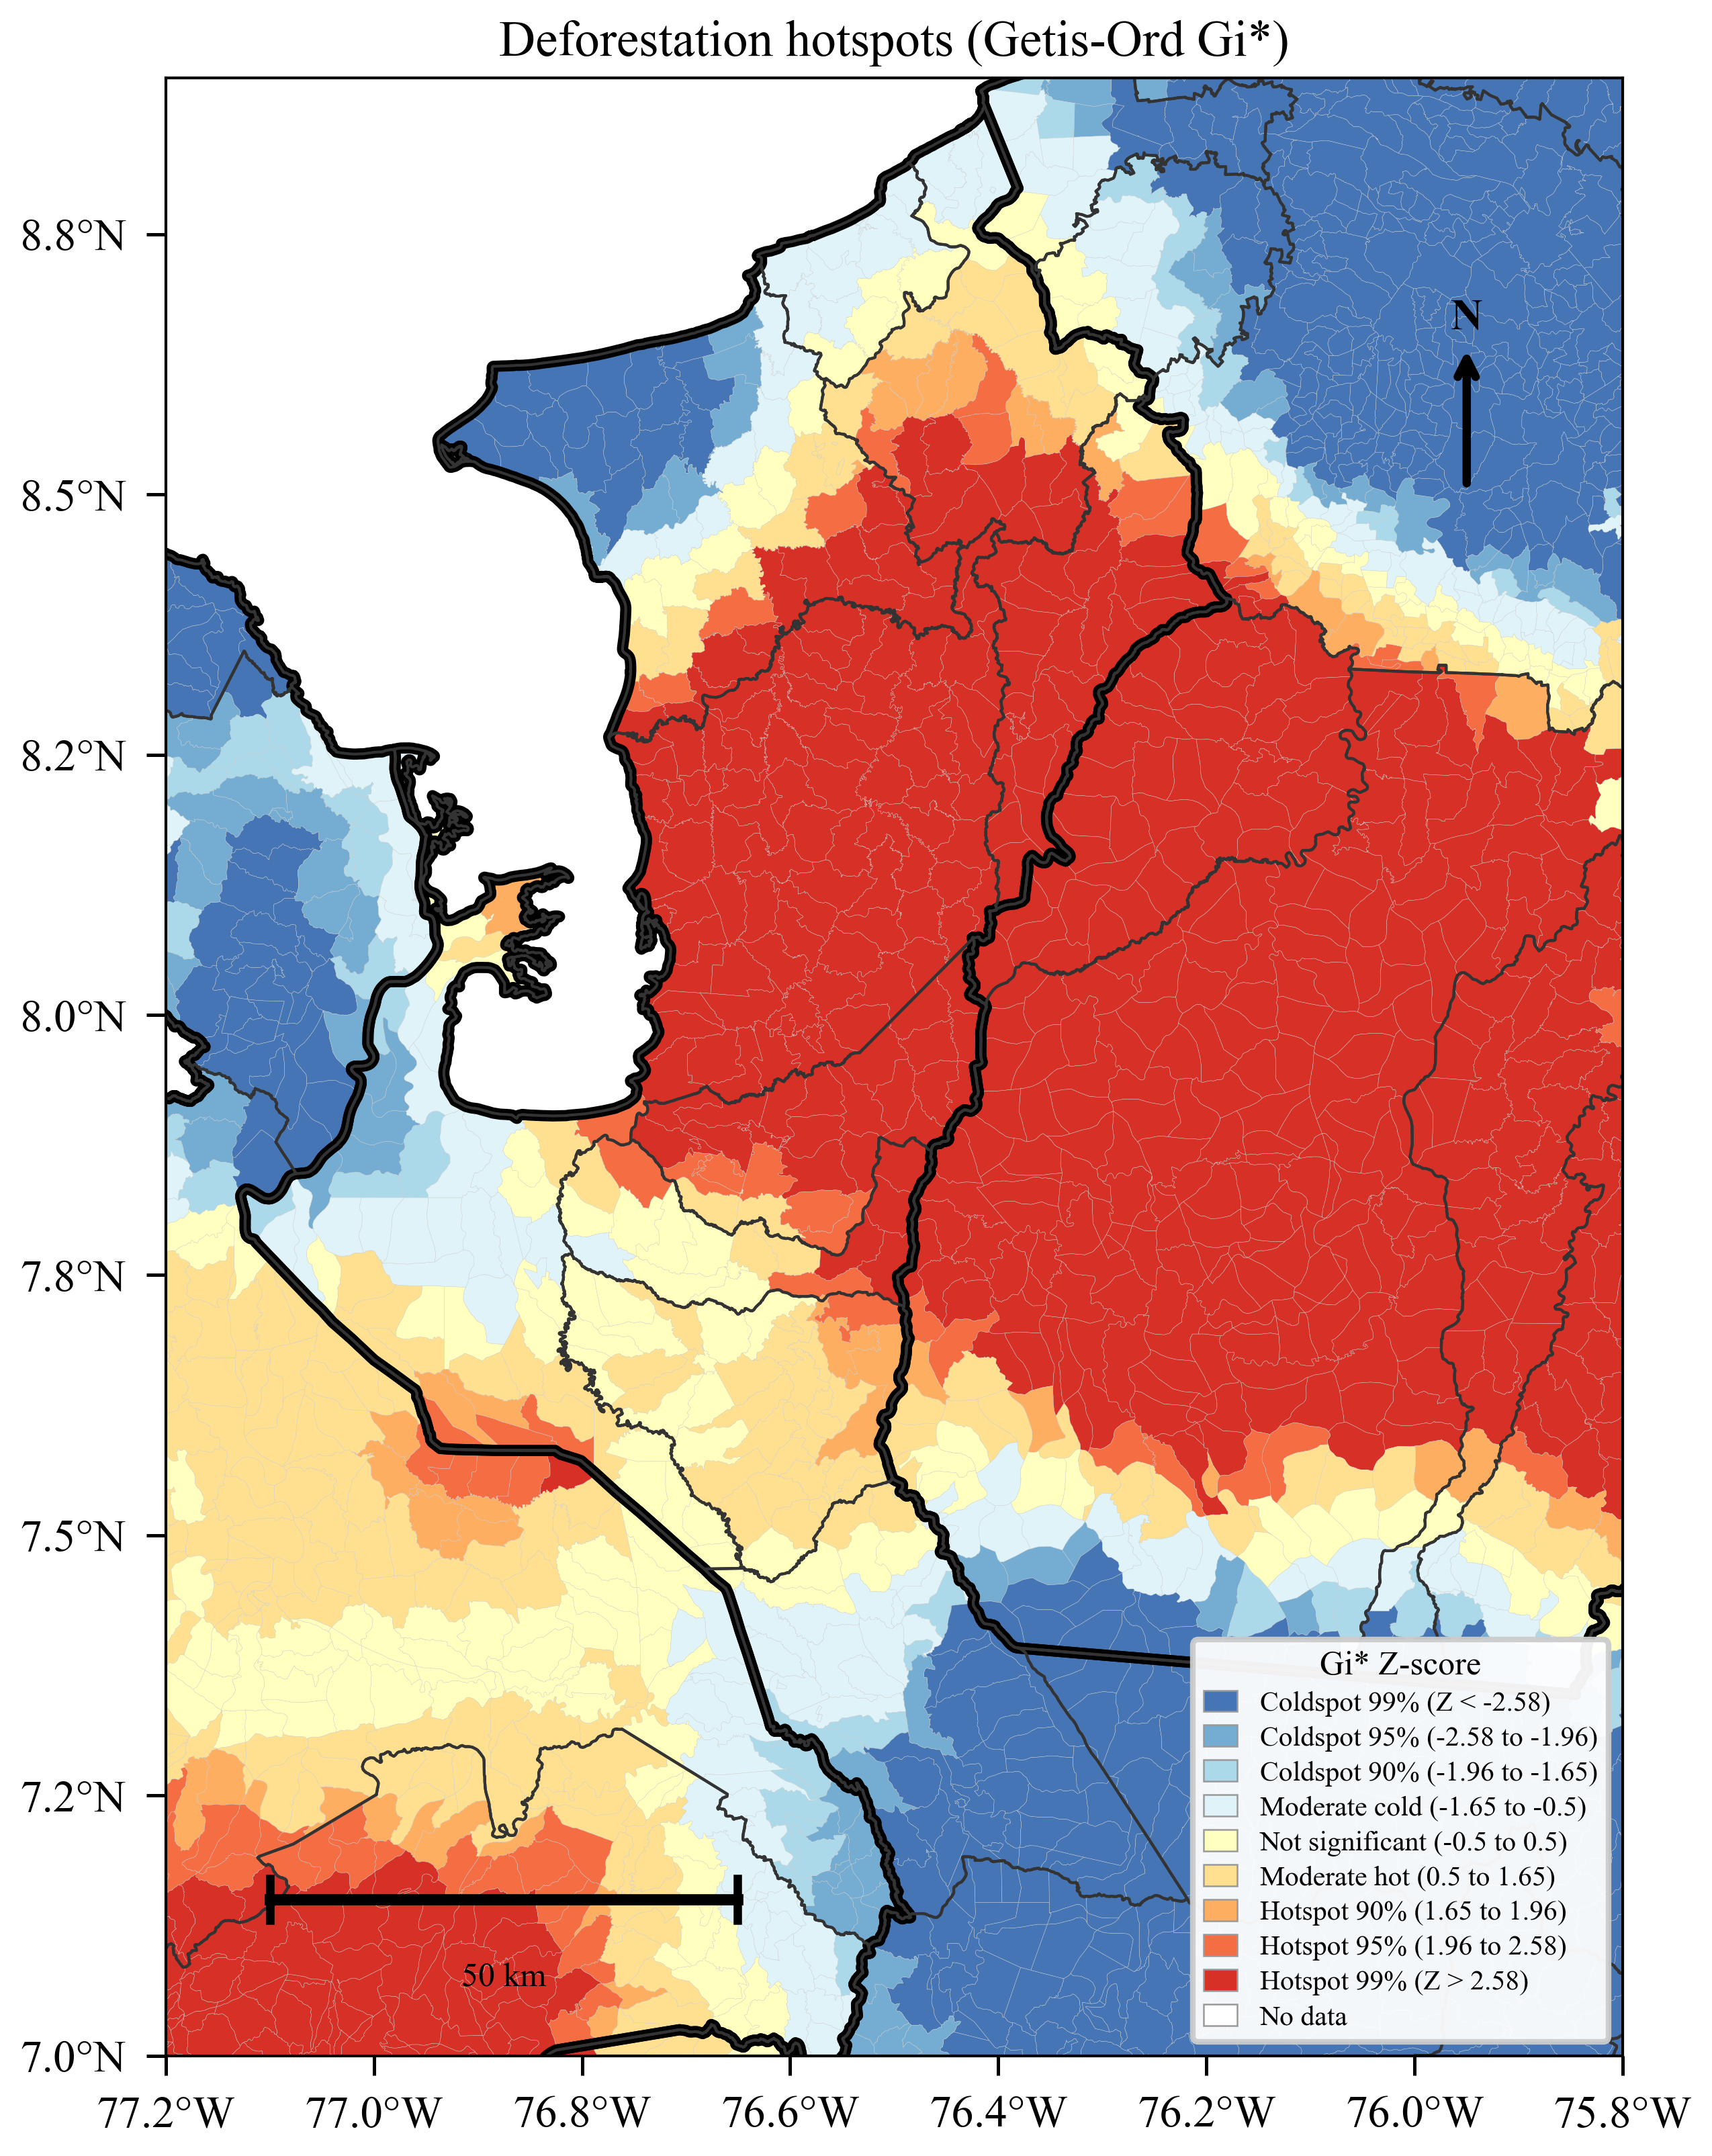
\includegraphics[width=\textwidth]{fig06_hotspot_choropleth.png}
\caption{Veredal-level deforestation hotspot choropleth (Getis-Ord Gi*). Dark red indicates hotspots ($\geq$2.58 Z-score, 99\% confidence), blue tones indicate coldspots. The eje bananero shows relative stability (coldspots) while deforestation frontiers in the Dari\'{e}n and southern zone show significant hotspot clustering.\label{fig:hotspots}}
\end{figure}

\subsection{Ecosystem Service Changes}

\subsubsection{Carbon Storage}

Using Tier~2 carbon densities calibrated for the Choc\'{o} bioregion \citep{Alvarez2012,Phillips2019}, total carbon stocks were estimated at 354.5~Tg~C (2013), 368.5~Tg~C (2016), 347.8~Tg~C (2020), and 315.1~Tg~C (2024) (Figure~\ref{fig:ecosystem}A)---a net decline of 39.4~Tg~C ($-$11.1\%) over the study period. Carbon stocks initially increased between T1 and T2 ($+$14.0~Tg~C) due to secondary forest expansion, then declined sharply: $-$20.7~Tg~C (T2$\rightarrow$T3) and $-$32.7~Tg~C (T3$\rightarrow$T4). Mangrove blue carbon contributed an estimated 19.5~Tg~C (T1) to 31.6~Tg~C (T4) to total stocks, with mangrove soil carbon alone accounting for 48.6\% of total mangrove carbon density.

The spatial distribution of carbon density and change is shown in Figure~\ref{fig:carbon_map}. The highest carbon densities were found in the Dari\'{e}n Chocoano (dense humid forest) and along the coastal mangrove belt, while the lowest values corresponded to the eje bananero and northern pasture areas.

\subsubsection{Water Yield}

Mean annual water yield was \num{2042}~mm (T1), \num{1937}~mm (T2), \num{1905}~mm (T3), and \num{2194}~mm (T4) (Figure~\ref{fig:ecosystem}C), reflecting the exceptionally high precipitation characteristic of the Choc\'{o} bioregion. Baseflow recharge was estimated at 491~mm (T1), 586~mm (T2), 518~mm (T3), and 745~mm (T4).

\subsubsection{Habitat Quality}

Mean habitat quality index was 0.195~(T1), 0.212~(T2), 0.200~(T3), and 0.247~(T4) (Figure~\ref{fig:ecosystem}D). The increase in T4 reflects the expansion of secondary forest and mangrove extent relative to T1. Mangrove habitat quality (0.9) contributed substantially to the regional index in coastal municipalities.

\begin{figure}[!ht]
\centering
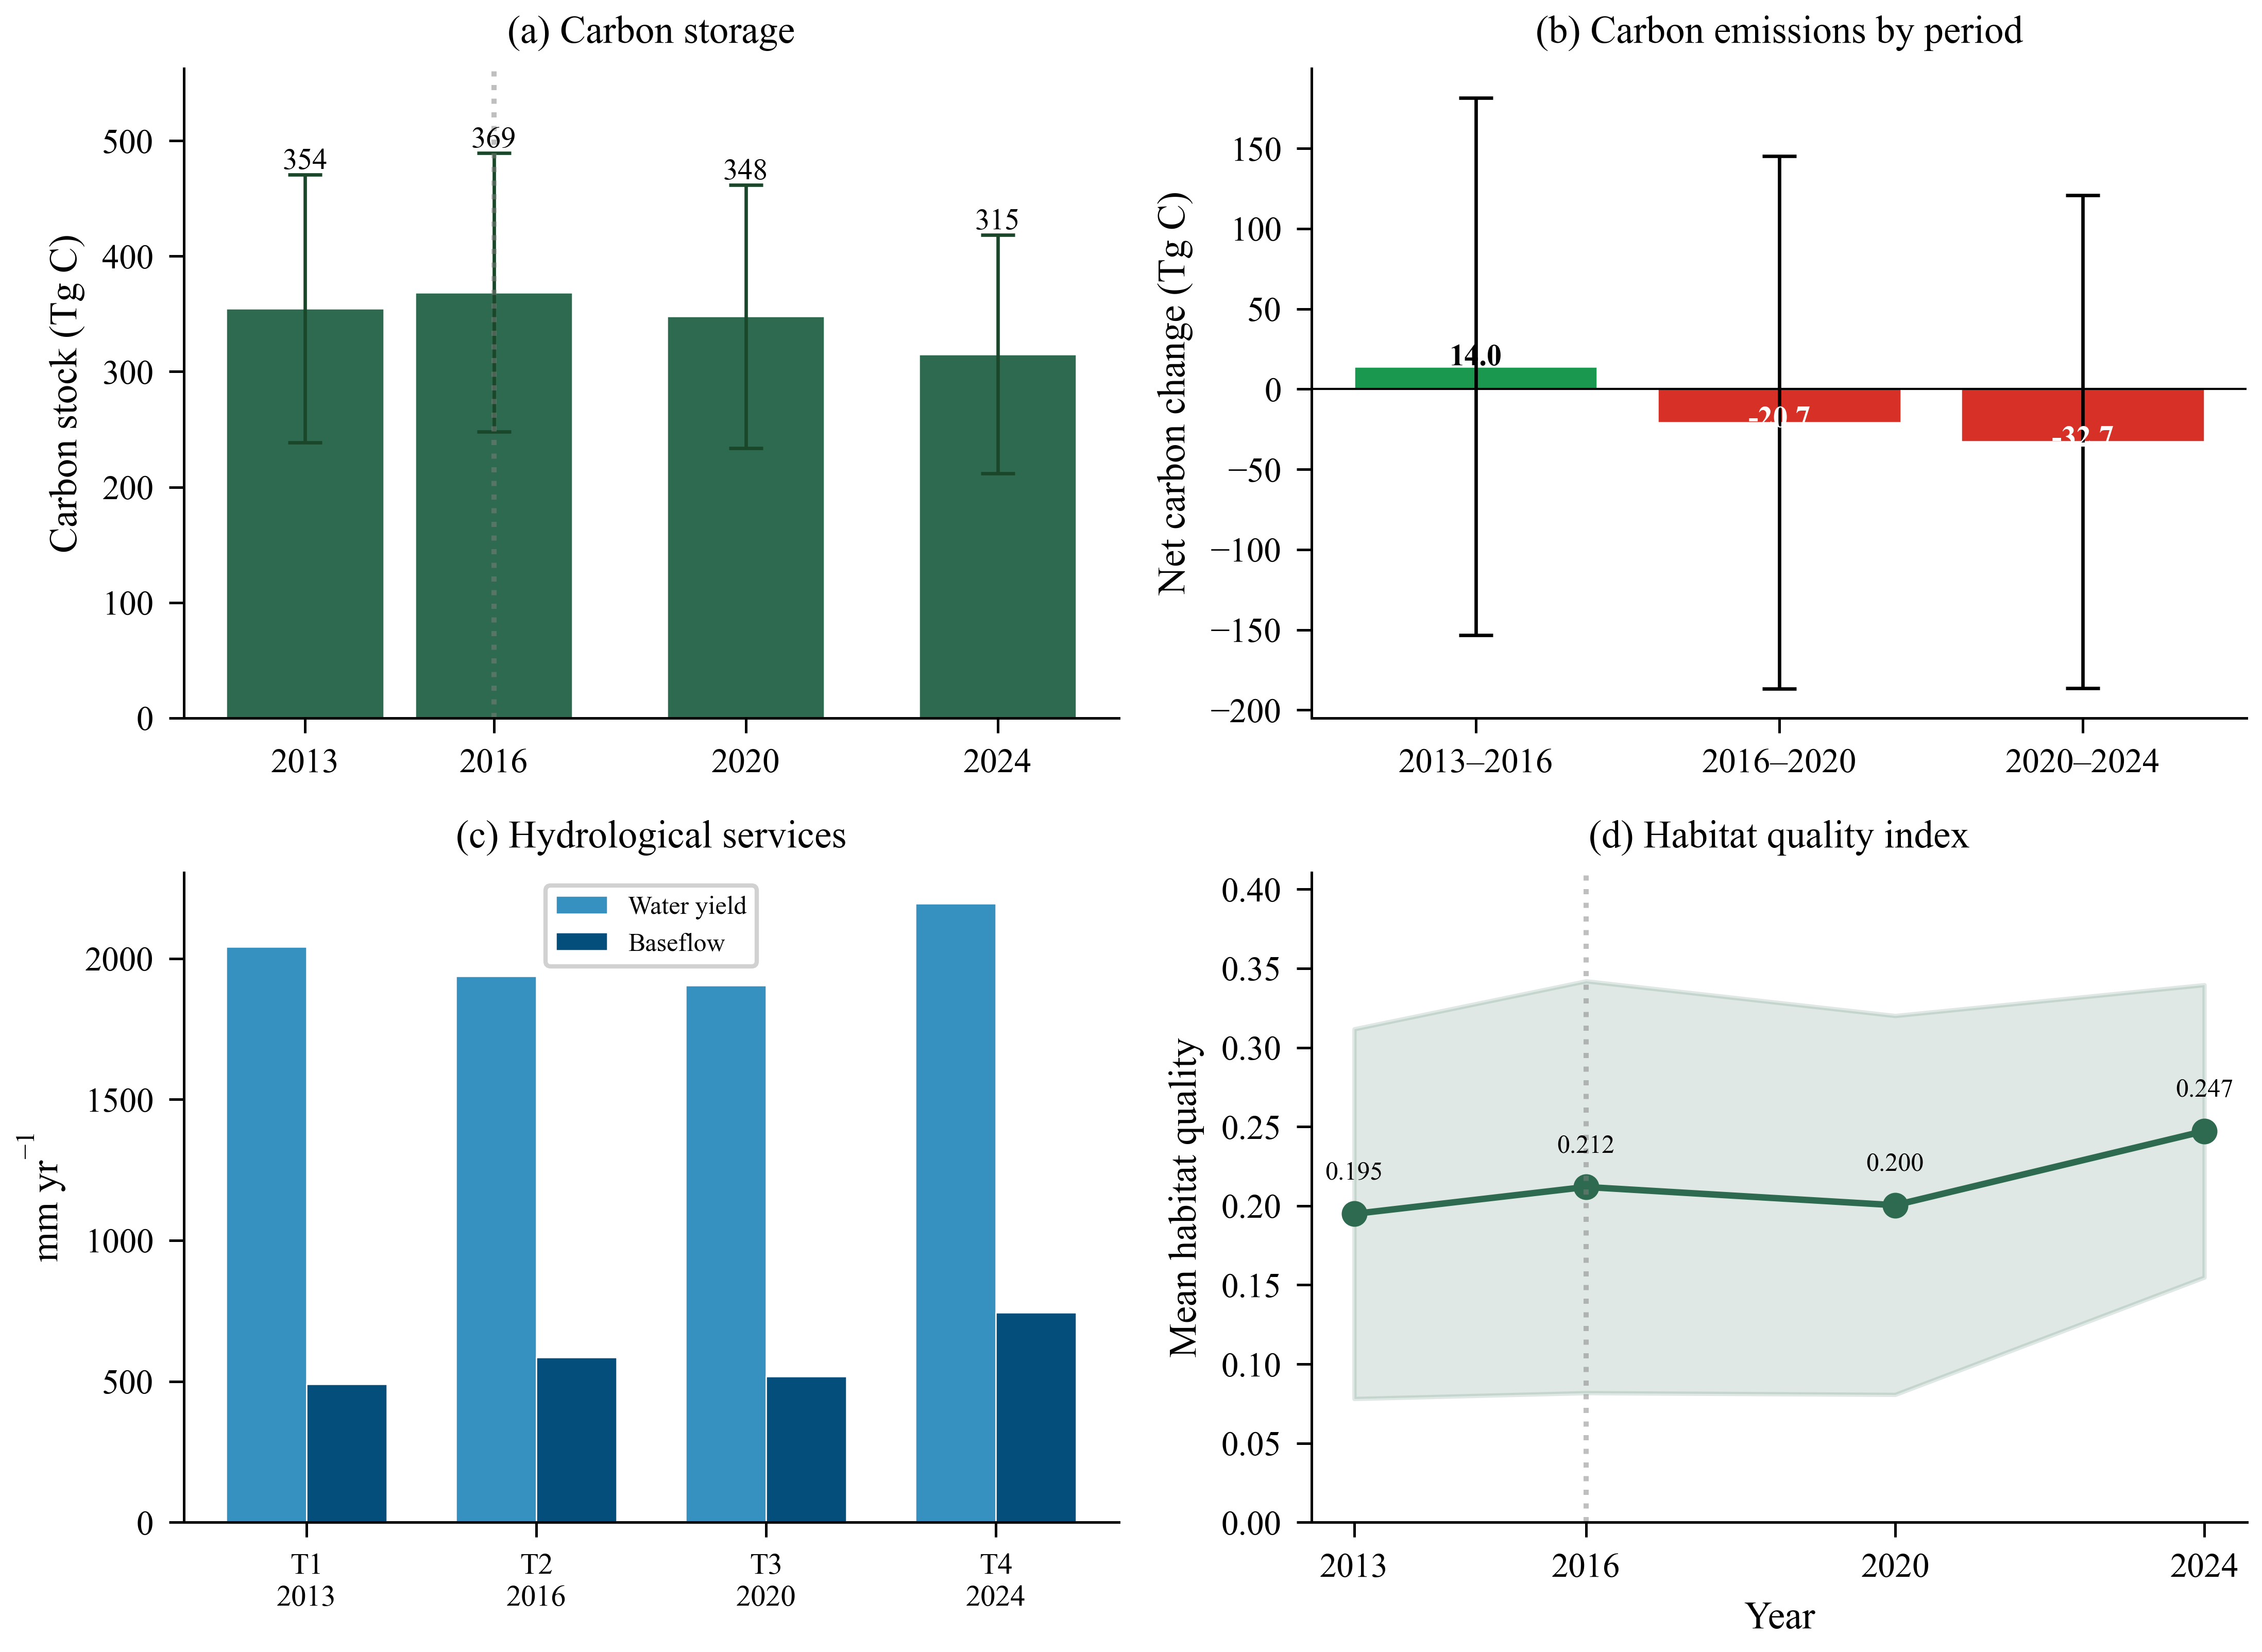
\includegraphics[width=0.7\textwidth]{fig08_ecosystem_services.pdf}
\caption{Ecosystem service changes: (A)~Carbon storage (Tier~2, Choc\'{o}-calibrated; \citealp{Alvarez2012,Phillips2019}) with propagated 95\% CI. (B)~Net carbon change by period with 95\% CI (including mangrove blue carbon). (C)~Hydrological services. (D)~Habitat quality index.\label{fig:ecosystem}}
\end{figure}

\begin{figure}[!ht]
\centering
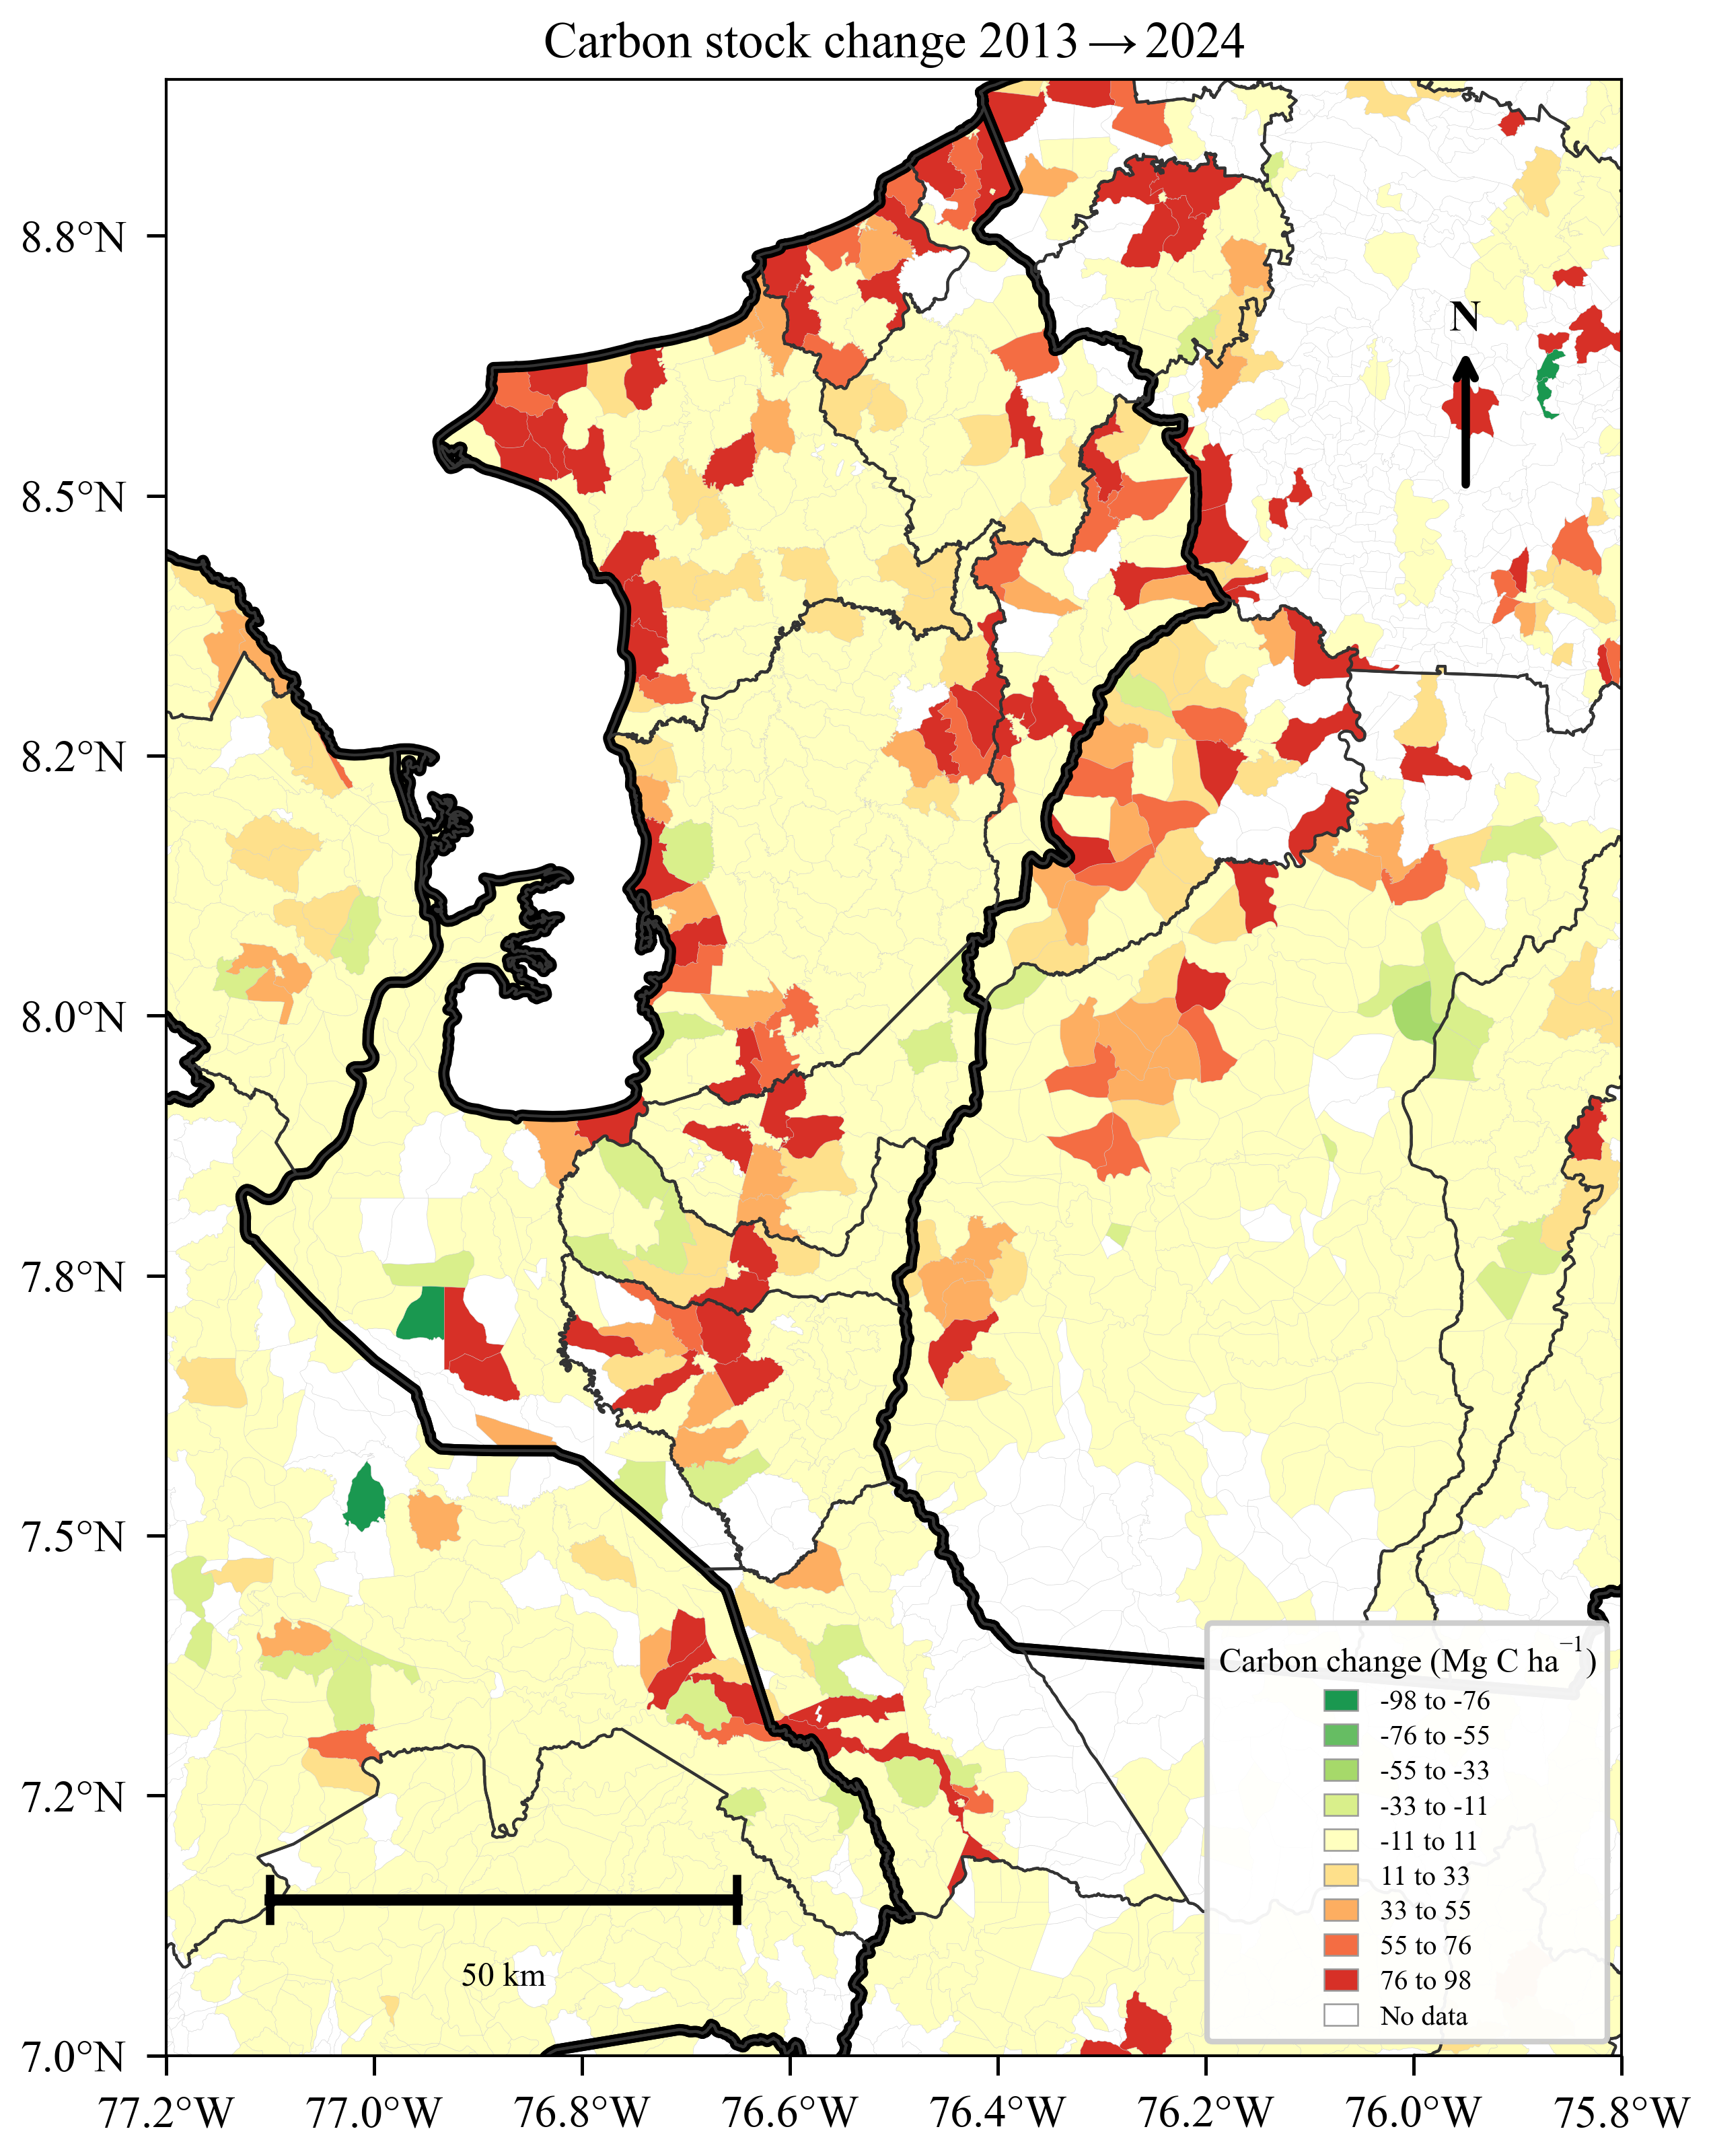
\includegraphics[width=\textwidth]{fig07_carbon_choropleth.png}
\caption{Veredal-level carbon stock change choropleth (2013--2024). Red indicates carbon loss (concentrated in deforestation frontiers), green indicates carbon gain (secondary forest recovery). Coastal mangrove zones show distinct carbon dynamics. Derived from 8-class LULC classification and Tier~2 Choc\'{o}-calibrated carbon pools.\label{fig:carbon_map}}
\end{figure}

\subsection{Drivers of Deforestation (GWR)}

The global OLS model explained 14.4\% of variance in deforestation rates (adjusted $R^2 = 0.138$; AIC~$= -2923$; $n = 1{,}287$). GWR with adaptive bisquare kernel (bandwidth~$= 12$ nearest neighbors) significantly improved model fit (mean local $R^2 = 0.426$; AIC~$= -7143$), confirming substantial spatial non-stationarity (H3). The AIC improvement of \num{4220} units strongly favors GWR over the global model.

Key OLS regression findings: elevation was a strong negative predictor of deforestation ($\beta = -0.144$, $t = -5.99$, $p < 0.001$), followed by LST ($\beta = -0.132$, $t = -5.14$), distance to roads ($\beta = 0.073$, $t = 5.17$), distance to urban centers ($\beta = 0.048$, $t = 4.09$), precipitation ($\beta = -0.042$, $t = -3.04$), distance to rivers ($\beta = -0.029$, $t = -2.40$), and clay content ($\beta = -0.025$, $t = -2.44$). Slope and population density were not significant at $\alpha = 0.05$. The spatial variation of GWR coefficients (Figure~\ref{fig:gwr}) reveals distinct driver regimes: in the eje bananero, proximity to existing plantations drives conversion, while in the Dari\'{e}n and southern montane zones, distance to roads and elevation are the dominant factors.

\begin{figure}[!ht]
\centering
\includegraphics[width=\textwidth]{fig10_gwr_choropleth_4panel.png}
\caption{Veredal-level GWR local coefficient choropleths for four key deforestation drivers. Veredas colored by interpolated local coefficient value using a divergent RdBu scale centered on zero. The eje bananero shows distinct driver patterns from the Dari\'{e}n frontier and southern montane zone.\label{fig:gwr}}
\end{figure}

\subsection{Future Scenarios}

CA-Markov projections (Figure~\ref{fig:scenarios}; Table~\ref{tab:scenarios}) show that under BAU, dense forest increases to 29.4\% by 2040 (from 21.3\% in 2024), reflecting the secondary forest$\rightarrow$dense forest recovery pathway embedded in the transition matrix. Under the conservation scenario, dense forest reaches 36.5\% by 2040---a 71.5\% increase from current levels. The PDET Urab\'{a} scenario---which models the combined effect of land restitution, sustainable agricultural practices, and mangrove restoration---projects 33.3\% dense forest and 32.3\% secondary forest by 2040 (total forest + mangroves: 66.6\%). Mangrove area declines under all scenarios (from 1.8\% to 0.9--1.1\% by 2040), indicating that the current transition dynamics favor mangrove-to-pasture conversion unless explicit restoration policies are implemented. Model validation (hindcast 2016$\rightarrow$2020 matrix to predict 2024) yielded a relative MAE of 52.5\%, indicating moderate predictive capacity.

\begin{table}[!ht]
\caption{CA-Markov projected land cover composition (\%) using ecologically corrected transition matrix.\label{tab:scenarios}}
\begin{threeparttable}
\begin{tabular*}{\textwidth}{@{\extracolsep{\fill}}lccccccccc@{\extracolsep{\fill}}}
\toprule
Scenario & Year & Dense & Sec. & Past. & Crops & Water & Urban & Bare & Mang. \\
\midrule
Current  & 2024 & 21.3 & 29.0 & 25.0 & 0.0 & 15.9 & 7.1 & 0.0 & 1.8 \\
BAU      & 2030 & 25.0 & 33.5 & 19.9 & 0.0 & 15.8 & 4.2 & 0.0 & 1.6 \\
BAU      & 2040 & 29.4 & 32.4 & 18.6 & 0.0 & 15.6 & 2.9 & 0.0 & 1.1 \\
Conserv. & 2030 & 27.2 & 36.3 & 15.6 & 0.0 & 15.8 & 3.6 & 0.0 & 1.6 \\
Conserv. & 2040 & 36.5 & 33.4 & 11.9 & 0.0 & 15.6 & 1.7 & 0.0 & 0.9 \\
PDET     & 2030 & 26.4 & 34.2 & 18.0 & 0.0 & 15.8 & 3.9 & 0.0 & 1.6 \\
PDET     & 2040 & 33.3 & 32.3 & 15.5 & 0.0 & 15.6 & 2.3 & 0.0 & 1.0 \\
\bottomrule
\end{tabular*}
\begin{tablenotes}
\item Source: BAU: business-as-usual (current rates persist). Conservation: deforestation $\times 0.5$, recovery $\times 1.3$, Kat\'{i}os NP buffer enforced, mangrove restoration. PDET: deforestation $\times 0.7$, land restitution + diversification $\times 1.2$.
\end{tablenotes}
\end{threeparttable}
\end{table}

\begin{figure}[!ht]
\centering
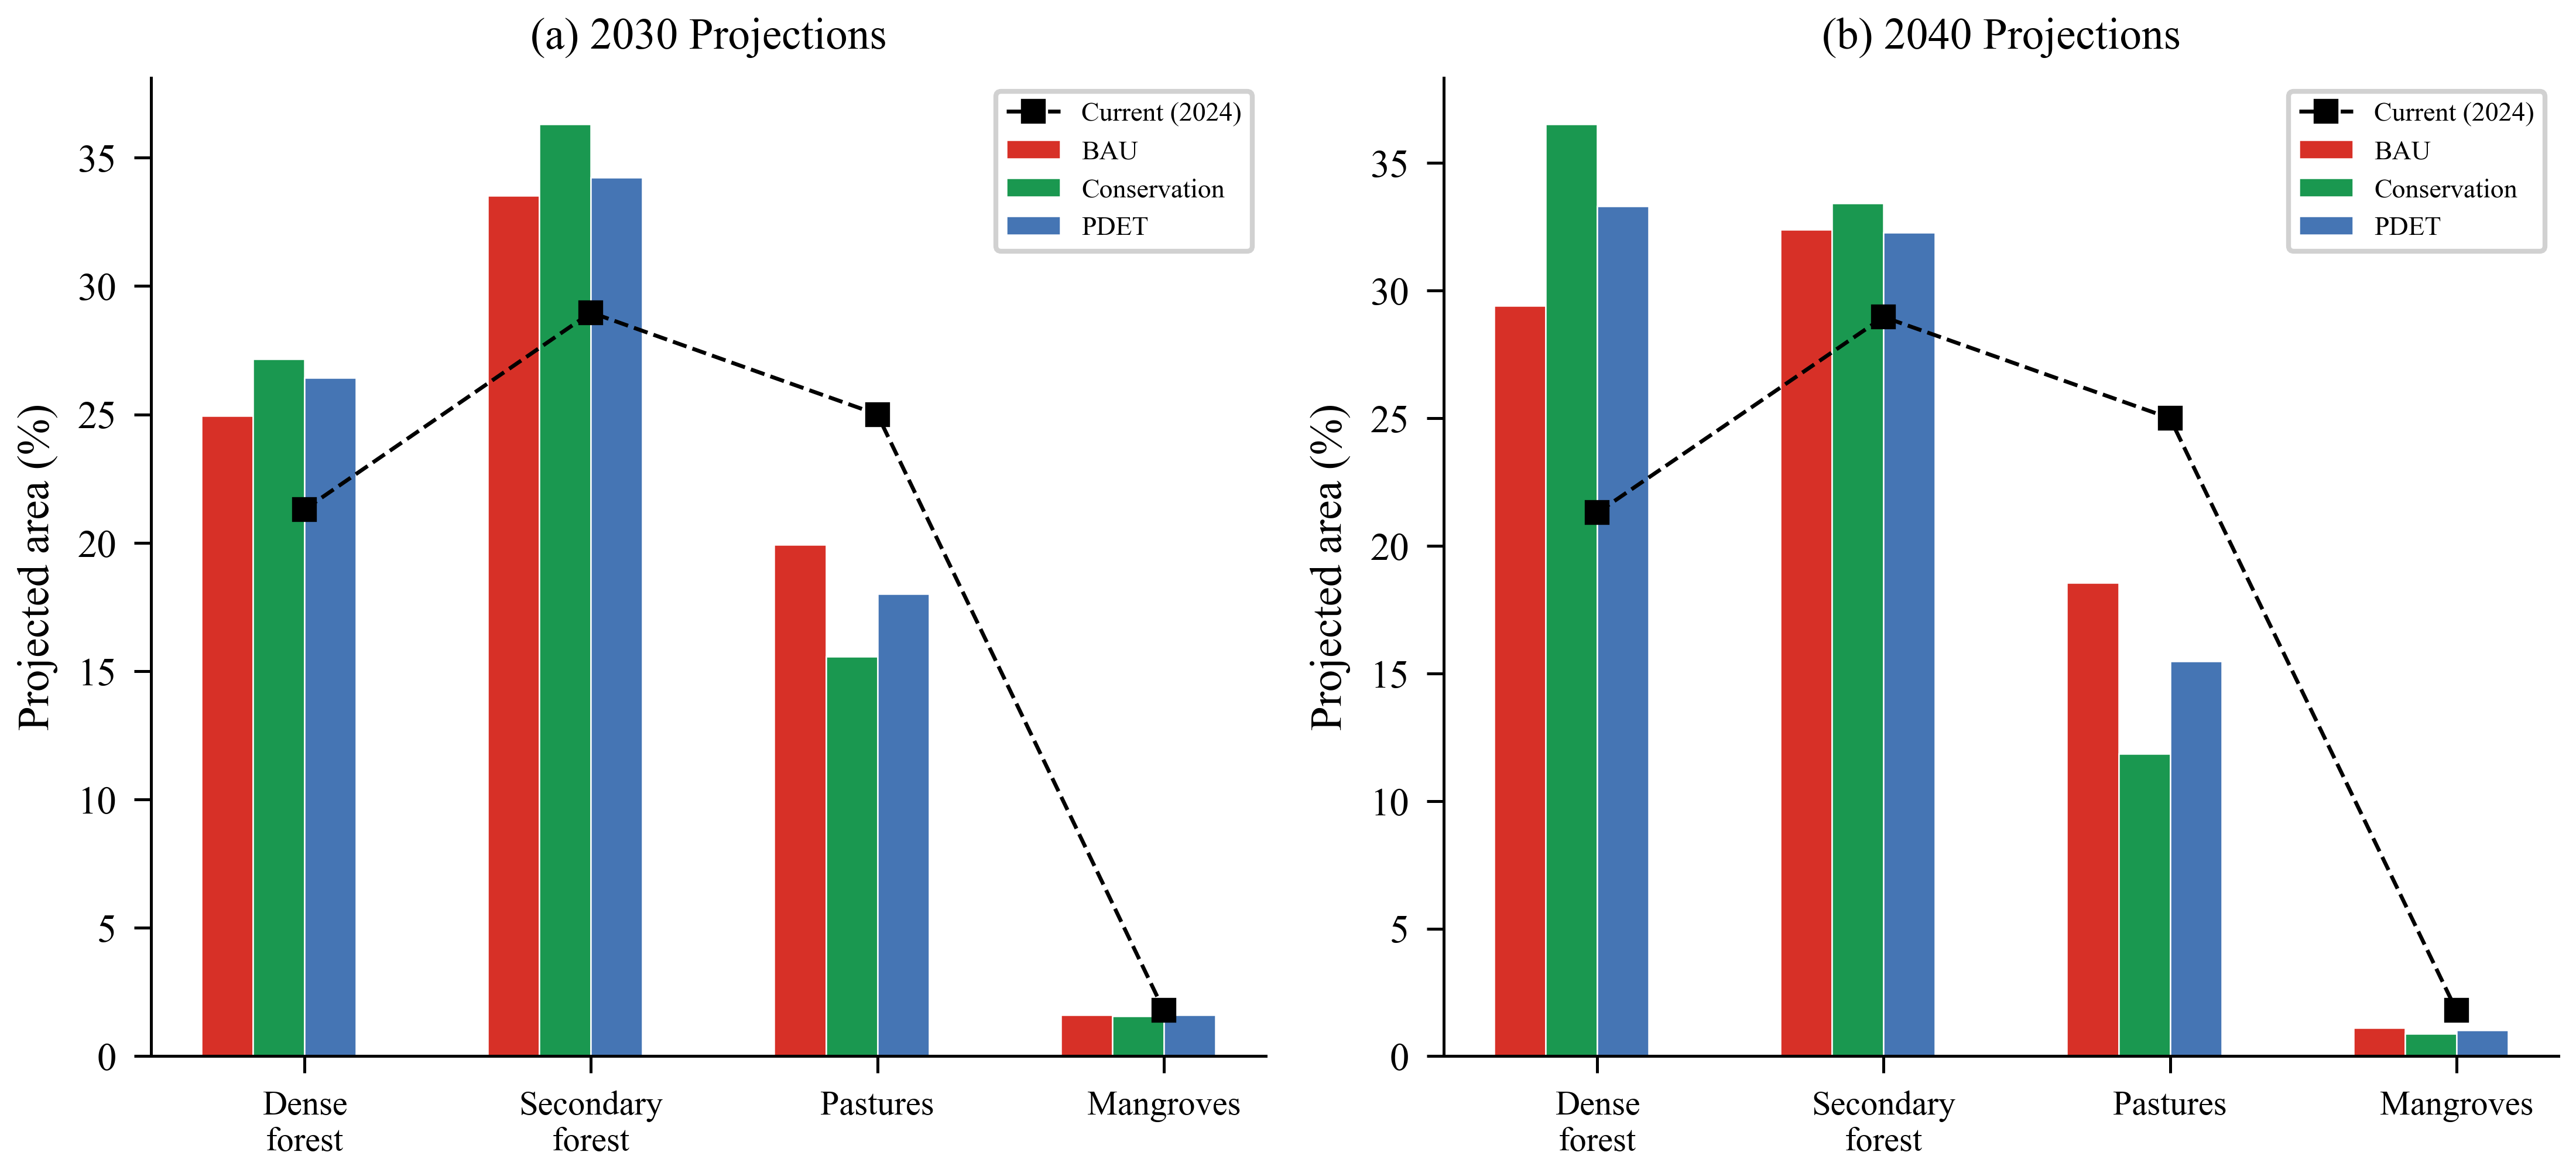
\includegraphics[width=0.7\textwidth]{fig11_camarkov_scenarios.pdf}
\caption{CA-Markov projected land cover composition under three scenarios for four key classes (dense forest, secondary forest, pastures, mangroves): (A)~2030 projections, (B)~2040 projections. Current (2024) baseline shown as dashed black line.\label{fig:scenarios}}
\end{figure}

\subsection{Climate Trends}

Mann-Kendall analysis revealed non-significant positive trends in annual precipitation (Kendall $\tau = 0.180$, $p = 0.44$; Sen's slope~$= +21.2$~mm~yr$^{-1}$) and non-significant negative trends in LST (Kendall $\tau = -0.168$, $p = 0.43$; Sen's slope~$= -0.036$$^\circ$C~yr$^{-1}$) over the 2012--2024 period (Figure~S2). Annual precipitation ranged from \num{2662}~mm (2020) to \num{3639}~mm (2022), while LST ranged from 27.0$^\circ$C (2022) to 28.6$^\circ$C (2015). The 2020 drought (SPI~$= -1.01$) coincided with the COVID-19 pandemic period, while 2024 showed above-average precipitation (SPI~$= +0.93$).


%%%%%%%%%%%%%%%%%%%%%%%%%%%%%%%%%%%%%%%%%%
\section{Discussion}
%%%%%%%%%%%%%%%%%%%%%%%%%%%%%%%%%%%%%%%%%%

\subsection{Forest Dynamics in Post-Conflict Urab\'{a}: Beyond the Amazonian Narrative}

Our findings extend the understanding of post-conflict environmental dynamics in Colombia beyond the well-studied Amazonian frontier \citep{Prem2020,Clerici2020,MurilloSandoval2021}. Urab\'{a} presents fundamentally different dynamics: rather than colonization-driven frontier deforestation, land use change here is shaped by an established agroindustrial economy, paramilitary-era land dispossession legacies, and the intersection of legal (banana, palm) and illegal (coca, mining) economic activities.

Using \citet{Olofsson2014} stratified area estimators, we estimate total forest cover (dense~$+$~secondary~$+$~mangroves) declined by approximately 7.2\% over the 2013--2024 period, driven primarily by a 39.3\% reduction in dense forest area. The spatial pattern of deforestation---concentrated in the Dari\'{e}n frontier and southern montane zone rather than in the already-converted eje bananero---suggests that deforestation in Urab\'{a} follows a ``development gradient'' pattern rather than simple frontier expansion. This finding is consistent with the observation by \citet{Armenteras2013,Armenteras2019} that Colombian deforestation patterns are increasingly driven by market integration and infrastructure rather than pure frontier colonization.

\subsection{Cross-Regional Comparison: Urab\'{a} vs.\ Magdalena Medio}

This study was designed to enable direct comparison with a parallel analysis of the Magdalena Medio region (Espinal Maya \& Jim\'{e}nez Londo\~{n}o, in preparation). Key differences emerge:

\begin{itemize}
\item \textbf{Carbon density:} Urab\'{a}'s Choc\'{o} forests hold approximately 22\% higher aboveground carbon than Magdalena Medio's inter-Andean forests (155 vs.\ 125~Mg~C~ha$^{-1}$), reflecting the exceptional biomass of the Choc\'{o} bioregion \citep{Phillips2019}. The addition of mangrove blue carbon further amplifies the ecosystem service value at stake.
\item \textbf{Conflict dynamics:} Magdalena Medio experienced overlapping FARC/ELN/paramilitary presence centered on petroleum infrastructure, while Urab\'{a}'s conflict was dominated by paramilitary consolidation (AUC) followed by successor groups (Clan del Golfo), with distinct implications for land tenure and restitution.
\item \textbf{Economic drivers:} The banana export industry in Urab\'{a} provides a more formalized economic base than the petroleum-cattle-coca economy of Magdalena Medio, potentially offering different pathways for sustainable development.
\item \textbf{Study area:} Urab\'{a} (${\sim}$11,000~km$^2$, 15 municipalities) is substantially smaller and more ecologically homogeneous than Magdalena Medio (${\sim}$36,800~km$^2$, 30 municipalities), but its coastal dimension adds ecological complexity absent in the inter-Andean valley.
\end{itemize}

\subsection{Mangrove Dynamics and Blue Carbon}

The explicit inclusion of mangroves as a distinct LULC class represents a methodological advance over binary forest/non-forest analyses. Mangrove ecosystems along the Gulf of Urab\'{a} and R\'{i}o Atrato estuary are globally significant for biodiversity and carbon storage \citep{BlancoLibreros2012,BlancoLibreros2015,Polidoro2010}. Our Tier~2 carbon estimates assign mangroves a total carbon density of 247~Mg~C~ha$^{-1}$, of which 120~Mg~C~ha$^{-1}$ is stored in soils---making mangrove conversion a disproportionately carbon-intensive land use change \citep{Donato2011,Twilley2018,Alongi2014}.

The complex trend in mangrove extent---increasing from \num{78770}~ha (T1) to \num{141736}~ha (T3) before declining to \num{127815}~ha (T4)---may reflect both genuine dynamics and classification variability associated with the multi-sensor approach. The net increase over the study period is consistent with regional studies documenting mangrove degradation from coastal development, aquaculture, and altered hydrology in the Gulf of Urab\'{a} \citep{Estrada2014,BlancoLibreros2015}. The conservation scenario's explicit mangrove restoration component underscores the outsized climate mitigation potential of coastal ecosystem protection.

\subsection{Ecosystem Service Implications}

Carbon stocks estimated using Choc\'{o}-calibrated Tier~2 values declined from 354.5 to 315.1~Tg~C ($-$11.1\%) over the study period. Per-hectare carbon density in Urab\'{a} ($281$~Mg~C~ha$^{-1}$ for dense forest, $247$ for mangroves) substantially exceeds national averages, confirming H2: ecosystem service losses per unit of deforestation are disproportionately high in this biodiversity hotspot. This has direct implications for REDD+ and blue carbon credit mechanisms, which should weight Choc\'{o} and mangrove deforestation more heavily than equivalent areas in less carbon-dense regions.

\subsection{The Migration Corridor Factor}

Urab\'{a} presents a unique dimension absent from other post-conflict LULC studies: its role as the primary transit corridor for irregular migration through the Dari\'{e}n Gap. Since 2019, hundreds of thousands of migrants annually traverse the Dari\'{e}n jungle, with environmental consequences that are only beginning to be documented: trail degradation, temporary settlement impacts, waste accumulation, and increased demand on local resources. While our satellite-based methodology cannot directly capture these impacts at 30~m resolution, the governance challenges posed by the migration crisis compound existing pressures on forest conservation and territorial planning.

\subsection{Policy Implications for PDET Urab\'{a}}

Our findings carry direct implications for post-conflict territorial planning in Urab\'{a}:

\begin{enumerate}[label=\arabic*.]
\item \textbf{Spatially targeted interventions:} Deforestation hotspots should be priority areas for enhanced governance, particularly in the Dari\'{e}n frontier and southern montane zone where institutional presence is weakest.
\item \textbf{Land restitution and environmental restoration:} The ${\sim}$40,000~ha subject to restitution claims represent an opportunity to integrate forest conservation into land tenure formalization.
\item \textbf{Mangrove conservation:} The Gulf of Urab\'{a} mangrove belt should be designated as a priority blue carbon conservation area, with enforceable buffer zones and restoration targets.
\item \textbf{Sustainable agroindustry:} The banana/palm sector's economic weight provides leverage for promoting deforestation-free supply chains and RSPO/Rainforest Alliance certification.
\item \textbf{Kat\'{i}os NP buffer:} Expanding the effective protection zone around PNN Los Kat\'{i}os could safeguard some of the highest-carbon forests in the study area.
\item \textbf{Cross-regional learning:} Comparing Urab\'{a} and Magdalena Medio outcomes provides evidence for adaptive management of PDET programs across different post-conflict contexts.
\end{enumerate}

\subsection{Methodological Considerations and Limitations}

Key limitations include:

\begin{enumerate}[label=\arabic*.]
\item \textbf{Cloud cover:} The Choc\'{o} bioregion's exceptionally high cloud cover (one of the cloudiest regions globally) limits the number of clear observations available for compositing, potentially reducing classification accuracy in the wettest municipalities.
\item \textbf{Classification accuracy:} Eight-class classification in a heterogeneous tropical landscape presents greater discrimination challenges than the 7-class system used in the Magdalena Medio. The Olofsson framework explicitly accounts for this uncertainty.
\item \textbf{Mangrove/water confusion:} Spectral similarity between mangroves and water in mixed-pixel coastal areas may introduce commission/omission errors for the mangrove class, mitigated by GMW cross-referencing.
\item \textbf{Banana/pasture confusion:} Banana plantations and improved pastures show similar NDVI signatures in certain seasons, potentially affecting crop/pasture discrimination.
\item \textbf{Carbon estimation:} While Choc\'{o}-calibrated Tier~2 values are used \citep{Phillips2019,Alvarez2012}, the high spatial variability of biomass in tropical humid forests introduces additional uncertainty. Site-specific Tier~3 measurements would further reduce this.
\item \textbf{Gulf of Urab\'{a}:} The Gulf's water area was masked but may skew area statistics in coastal municipalities if the coastline polygon is imprecise.
\item \textbf{Field access:} The persistence of armed groups (Clan del Golfo) and difficult terrain in the Dari\'{e}n limit field verification possibilities.
\item \textbf{GWR complexity:} As in the Magdalena Medio study, GWR ENP/$n$ ratios should be evaluated critically. Multiscale GWR \citep{Oshan2019} is recommended for future refinement.
\end{enumerate}


%%%%%%%%%%%%%%%%%%%%%%%%%%%%%%%%%%%%%%%%%%
\section{Conclusions}
%%%%%%%%%%%%%%%%%%%%%%%%%%%%%%%%%%%%%%%%%%

This study provides the first comprehensive multi-temporal analysis of land use and land cover change in Colombia's Urab\'{a} Antioque\~{n}o region, spanning the critical pre- to post-peace agreement period (2013--2024) with an eight-class scheme explicitly capturing mangrove dynamics. Our key findings are:

\begin{enumerate}[label=\arabic*.]
\item Estimated total forest cover (dense~$+$~secondary~$+$~mangroves) declined by 7.2\% over the study period, with dense forest experiencing a 39.3\% reduction (\num{740642}$\rightarrow$\num{449476}~ha). Dense forest-to-pasture conversion was the dominant transition (\num{331960}~ha in T3$\rightarrow$T4 alone), concentrated in the Dari\'{e}n frontier and southern montane zone rather than the already-converted eje bananero (H1 supported).
\item Carbon stocks declined from 354.5 to 315.1~Tg~C ($-$11.1\%), with per-hectare losses exceeding national averages due to the exceptionally high biomass of the Choc\'{o} bioregion (281~Mg~C~ha$^{-1}$ for dense forest, 247 for mangroves). Mangrove blue carbon contributed 19.5--31.6~Tg~C to regional stocks (H2 supported).
\item GWR ($R^2 = 0.426$, AIC improvement of \num{4220} over OLS) revealed spatially varying deforestation drivers, with distinct regimes in the eje bananero (agroindustrial expansion), the Dari\'{e}n frontier (road access/colonization), and the southern montane zone (elevation/cattle ranching) (H3 supported).
\item CA-Markov projections show dense forest recovering to 29.4\% under BAU by 2040, with the conservation scenario reaching 36.5\% and the PDET scenario 33.3\%. However, mangroves decline under all scenarios (from 1.8\% to 0.9--1.1\%) unless explicit restoration policies are implemented (H4 partially supported).
\item The inclusion of a dedicated mangrove class and Choc\'{o}-calibrated carbon pools provides more accurate ecosystem service estimates for this biodiversity hotspot than generic national values.
\end{enumerate}

These findings, reported with full uncertainty bounds following \citet{Olofsson2014} stratified estimation, provide critical inputs for PDET Urab\'{a} territorial planning, land restitution programs, and blue carbon conservation strategies. The fully reproducible, GEE-based methodology enables cross-regional comparison with other post-conflict zones---including the Magdalena Medio---and offers a scalable framework for monitoring Colombia's post-conflict environmental transitions.


%%%%%%%%%%%%%%%%%%%%%%%%%%%%%%%%%%%%%%%%%%
%% Back matter
%%%%%%%%%%%%%%%%%%%%%%%%%%%%%%%%%%%%%%%%%%

\section*{Data Availability}
Google Earth Engine scripts are available upon request from the corresponding author (GEE project: ee-maestria-tesis). LULC classified maps and statistical outputs are available in the project repository.

\section*{Acknowledgments}
Google Earth Engine cloud computing resources were provided through the ee-maestria-tesis project. We thank the developers of GEE, CHIRPS, MODIS, Landsat, Sentinel-2, Hansen GFC, and Global Mangrove Watch datasets for open access to satellite-derived products.

\section*{Software}
Google Earth Engine \citep{Gorelick2017}, Python 3.x,
mgwr \citep{Oshan2019}, PySAL, scikit-learn, matplotlib, rasterio,
geopandas, rasterstats.

% Print bibliography
\printbibliography

\end{document}
